\documentclass[12pt]{article}
\usepackage{graphicx}
\usepackage{siunitx}
\usepackage{authblk}
\usepackage{amsmath}
\usepackage{booktabs} % for much better looking tables
\usepackage{array} % for better arrays (eg matrices) in maths
\usepackage{verbatim} % adds environment for commenting out blocks of text & for better verbatim
\usepackage{subfig} % make it possible to include more than one captioned figure/table in a single float
\usepackage{url}
\usepackage[parfill]{parskip}
\usepackage[top=1in, bottom=1in, left=0.9in, right=0.9in]{geometry}
\geometry{letterpaper}
\usepackage{mathptmx}
\usepackage{lineno}
\linenumbers
\usepackage[T1]{fontenc}
\usepackage{amsmath}
\numberwithin{equation}{section}
% \usepackage[numbers]{natbib}
% \usepackage{fancyvrb}
%\usepackage{lineno}
\usepackage{cleveref}
\usepackage{natbib}
\bibliographystyle{abbrvnat}
\setcitestyle{authoryear,open={(},close={)}}

\usepackage{pdflscape}
% \newcommand{\beginsupplement}{%
%         \setcounter{table}{0}
%         \renewcommand{\thetable}{S\arabic{table}}%
%         \setcounter{figure}{0}
%         \renewcommand{\thefigure}{S\arabic{figure}}%
%      }
    
\renewcommand{\thetable}{S\arabic{table}}%
\renewcommand{\thefigure}{S\arabic{figure}}%

\begin{document}
% \beginsupplement


\section{Development and analysis of trophic mode model}

\subsection{Description of the model and heterotrophy index}
We used a variable selection algorithm and Random Forest machine learning model framework in order to predict the likely trophic mode of the eukaryotic TOPAZ MAGs described in this study. Transcriptomes from the MMETSP and EukProt were manually-annotated as phototroph, mixotroph, or heterotroph based on the literature (Supplemental Table X). We tested our model with a randomly subset test set comprised of the 25\% of MMETSP and EukProt transcriptomes \citep{Keeling2014,Richter2020EukProt} that were excluded from the model building procedure. With this test subset we obtained an accuracy of 94.6\% (Supplemental Figure \ref{fig:confusionmatrix}), meaning that nearly 95\% of taxonomic annotations derived from the machine learning model aligned with their manually-assigned trophic mode annotation (\Cref{fig:confusionmatrix}).  When applied to the TOPAZ MAGs, all MAGs were either classified as phototrophs or heterotrophs, with none classified as  mixotrophs. This likely reflects that the model was generally conservative when it came to assigning genomes or transcriptomes as mixotrophs (\Cref{fig:mag-burns}). As a consequence, we developed a secondary metric for assessing the extent of heterotrophy in the test genomes and transcriptomes using the KOs selected by the vita selection process, but instead of using the presence or absence of these KOs as a binary indicator to inform the classification of the MAGs, we used the presence or absence as part of an equation to more sensitively assess the number of KOs present that tend to be indicative or either heterotrophy or phototrophy. The result was the ``Heterotrophy Index'', a metric for assessing trophy based on KEGG pathway presence or absence. 

The Heterotrophy Index is a sliding scale that weights the presence of heterotrophy, phototrophy- and mixotrophy-indicative KOs to assess the overall likely trophic state of an organism, and will consequently better show when an organism is more likely mixotrophic or possessing traits from both heterotrophy and phototrophy. Because mixotrophs were less common in our test dataset, there are natural concerns about the skill of the model when it comes to identifying them [ADD CITATION FOR UNEVEN TRAINING IN RF?]. Because the majority of test and training transcriptomes were phototrophs or heterotrophs, it is more conservative for a Random Forest model to assign these modes more frequently. As the TOPAZ MAGs covered lineages with known mixotrophic members [CITATION], and with comparison and feedback from an alternative trophic model as described in \Cref{burnssec}, we applied the Heterotrophy Index to provide more sensitivity in the identification of likely mixotrophs. In particular, with the Random Forest design, if a MAG has characteristics of both heterotrophs and phototrophs that are present in the training data, but does not align with the limited sample of mixotroph transcriptomes (which is also problematic due to the opportunistic nature of the sampling, see  \Cref{limitations}), these MAGs would be assigned the best guess between phototrophy and heterotrophy, when in reality this combination of traits may indicate some form of mixotrophy. The Heterotrophy Index also serves as a confidence metric for the trophy estimate. For example, a MAG with a large positive  Heterotrophy Index would more confidently be called a heterotroph, as this would indicate a strong frequency and degree of alignment with heterotroph references (and, specifically, alignment with those heterotrophic references for KOs identified by the vita algorithm as important for distinguishing trophic mode within the training set). By contrast, a small (or near zero) positive Heterotrophy Index may be mixotrophic or represent a less complete MAG. 

\subsection{Comparison to Burns and Lambert models}\label{burnssec}
In order to assess the performance of our model, which relies solely on assessment of KOs \citep{Kanehisa_2019} that were determined computationally to be important and assessed for function after the fact (\Cref{fig:ko-trophy}), we applied the model from \cite{burns2018gene} (heretofore referred to as the Burns model) to the same highly complete eukaryotic MAGs, as well as to the MMETSP transcriptomes. This model assigns a score from zero to one for individual characteristics related to trophy, including photosynthetic ability, phagocytosis, and prototrophy \citep{burns2018gene}. Using Hidden Markov Models for selected genes which have known association with the afore mentioned trophic strategies, the Burns model instead looks for a set of genes consistent with each trait, to assess the ``completeness'' of the genome or transcriptome with respect to the machinery known to be involved with each function. We found the Burns model results to be consistent with our heterotrophy index procedure in the following ways. Among the MMETSP transcriptomes, XX\% (n=XX) of the transcriptomes with a positive Heterotrophy Index (indicative of net heterotrophy) also had a photosynthesis score of less than 0.5 as assigned by the Burns model, and XX\% (n=XX) had a photosynthesis score of less than 0.05 via the Burns model (Figure \ref{fig:mmetsp-burns}). Similarly, XX\% (n=XX)  of MMETSP transcriptomes with a negative heterotrophy index (indicative of net phototrophy) had a photosynthesis score of greater than 0.5 as assigned by the Burns model. MMETSP transcriptomes with a zero or near-zero heterotrophy index, which corresponds to putative mixotrophy, had varying photosynthesis scores according to the Burns model, but were more likely to have high (0.6-1) photosynthesis scores, which is consistent with mixotrophy (Figure \ref{fig:mmetsp-burns}). However, several of the MAGs which were predicted to be mixotrophs by the Random Forest model and were annotated manually as mixotrophs from the available metadata had mid- to high- photosynthesis scores in the Burns model, yet negative-leaning Heterotrophy Index scores. These transcriptomes also tended to have high (>0.7) phagocytosis predictions per the Burns model, consistent with the presence of genetic resources for both heterotrophic and phototrophic strategies. Broadly, we found that, similarly to our heterotrophy index and Random Forest model annotations, the Burns photosynthesis prediction results tended to align with the expected lifestyle of each MAG based on EUKulele \citep{Krinos2021EUKulele} taxonomic annotations, with expected heterotrophs like amoebozoa, fungi, and opisthokonta scoring low on photosynthetic ability, while expected phototrophs like ochrophyta and chlorophyta tended to score highly for photosynthetic ability (Figure \ref{fig:mmetsp-burns}). Most disagreement was found within the SAR clade and Crypophyta, wherein a range of photosynthesis scores were found by the Burns model, and sometimes these scores contradicted the annotation found by the heterotrophy index and Random Forest model (Figure \ref{fig:mmetsp-burns}). This would indicate potentially cryptic and variable trophic strategies and lifestyles within these annotated groups. 

When split into classes of photosynthetic ability based on Burns model scores, MMETSP transcriptomes with ``no'' photosynthesis according to the Burns model (photosynthesis prediction $<0.1$) had an average Heterotrophy Index of $38.85\pm68.19$, while transcriptomes with ``high'' photosynthesis (photosynthesis prediction $>0.9$) had an average Heterotrophy Index of $-272.34\pm119.94$ (\Cref{fig:burns-cats}). As far as the TOPAZ MAGs, we similarly found that the MAGs predicted to be heterotrophic had low variance in photosynthesis prediction as reported by the Burns model, yet the variability in the photosynthetic prediction was high, in particular among those MAGs of higher (less negative, hence closer to ``mixotrophic'') Heterotrophy Index (\Cref{fig:mag-burns}). 

\subsection{The future of trophic mode models}\label{limitations}
The model we developed relies solely upon references that were derived from expression-level data (transcriptomics). Additionally, we used the entire MMETSP \citep{Keeling2014} and EukProt \citep{Richter2020EukProt} databases with manually assigned trophic strategies based on the literature (SI Table X). Both of these choices carry issues that may be responsible for our under prediction of mixotrophy. First, as they were transcriptomic datasets, the experimental conditions that were used to generate the reference transcriptome are important, in that if a culture was maintained in phototrophy-favorable conditions (e.g. high light, sufficient inorganic nutrients) as opposed to heterotrophy-favorable conditions (e.g. low light, external carbon source), the transcripts reconstructed from these experiments  may result in a reference that is skewed towards phototrophy or heterotrophy, respectively. Regardless of the conditions in which the organism was grown, it is likely that genes present in the genome of the organism were not recovered by transcriptomics. While this means that important genes related to trophic strategy may be missed from the prediction workflow, this is also exciting, as there is much room for growth for these already accurate and skillful models. As genomic references become available and the number of transcriptomic experiments continue to grow, we can expect to further constrain the classes of genes that decide trophic mode. As databases grow, they may be pruned to include only experiments in which the trophy of the organism was known exactly, which would enable the patterns of expression which decide trophic mode to be  pinpointed more precisely. Ideally, a complete core set of protein families necessary for heterotrophy and for phototrophs could be identified. A fundamental question that remains, however, is if there are any genes or protein families that are characteristic of mixotrophic organisms \textit{only} or if these organisms are better characterized based on the co-occurrence of genes indicative of phototrophy and heterotrophy. If the latter,  mixotrophy would be best characterized by the proportion of these sets which overlap in the genome or the expression profile of the candidate organism. While this is in principle the aim of the Burns model (\cite{burns2018gene}, Section \ref{burnssec}), this approach might still  be augmented by machine learning-based techniques that have the capacity to identify important genes that may not have yet been annotated. 

\section*{Supplementary Figures}

\begin{landscape}
\begin{figure}
    \centering
    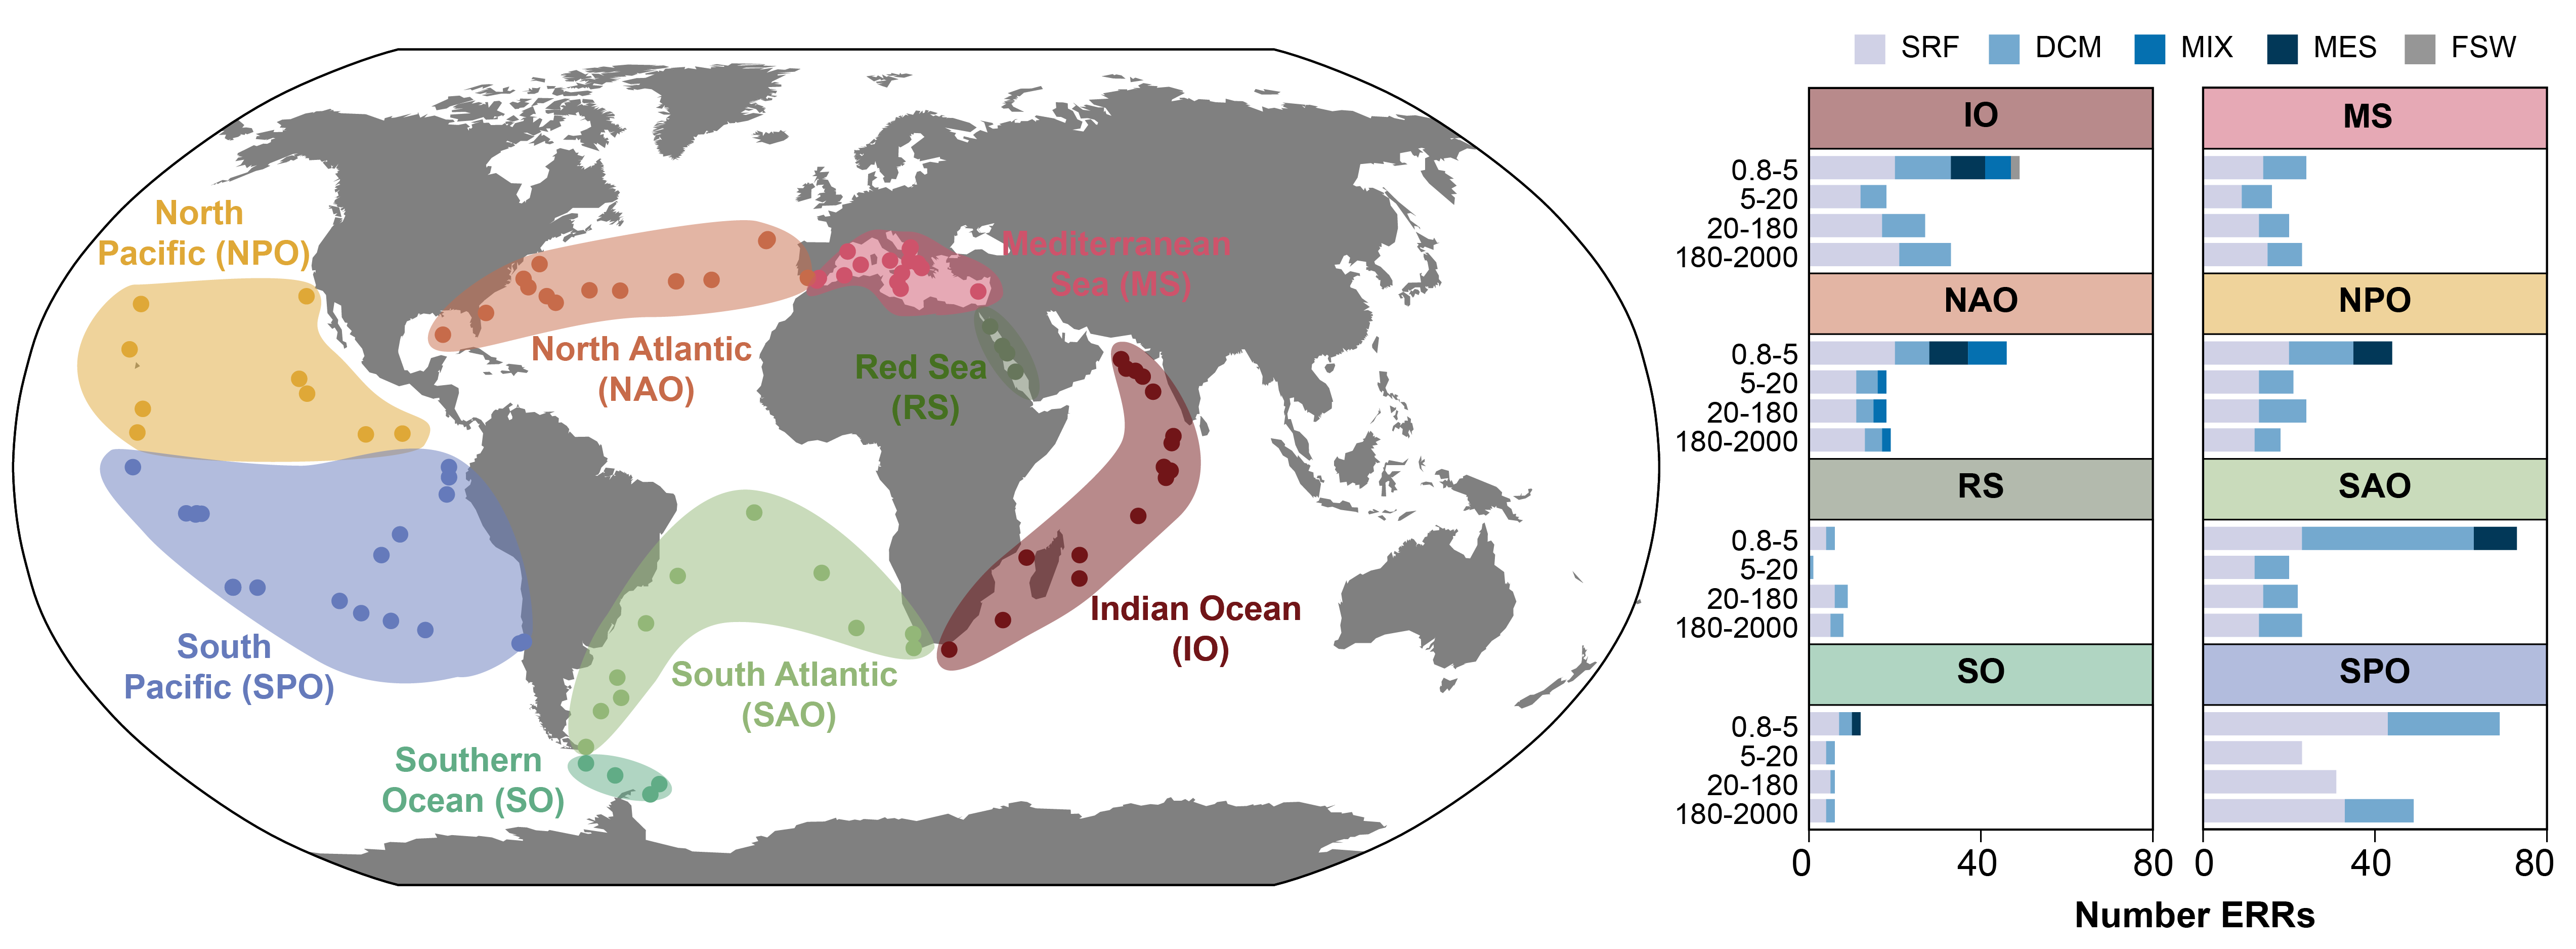
\includegraphics[width=0.95\columnwidth]{si-figures/Tara_stationMap-01.png}
    \caption{Sample map and distribution of sequence data sets across regions. Stations from Tara Oceans were categorized into general regions which are highlighted by color. The depth (surface (SRF), deep chlorophyll max (DCM), mixed surface sample (MIX), mesopelagic (MES), and filtered seawater (FSW) and size fraction are shown as bar plots for each ocean region. }
    \label{fig:tara-map}
\end{figure}
\end{landscape}

\begin{figure}
    \centering
    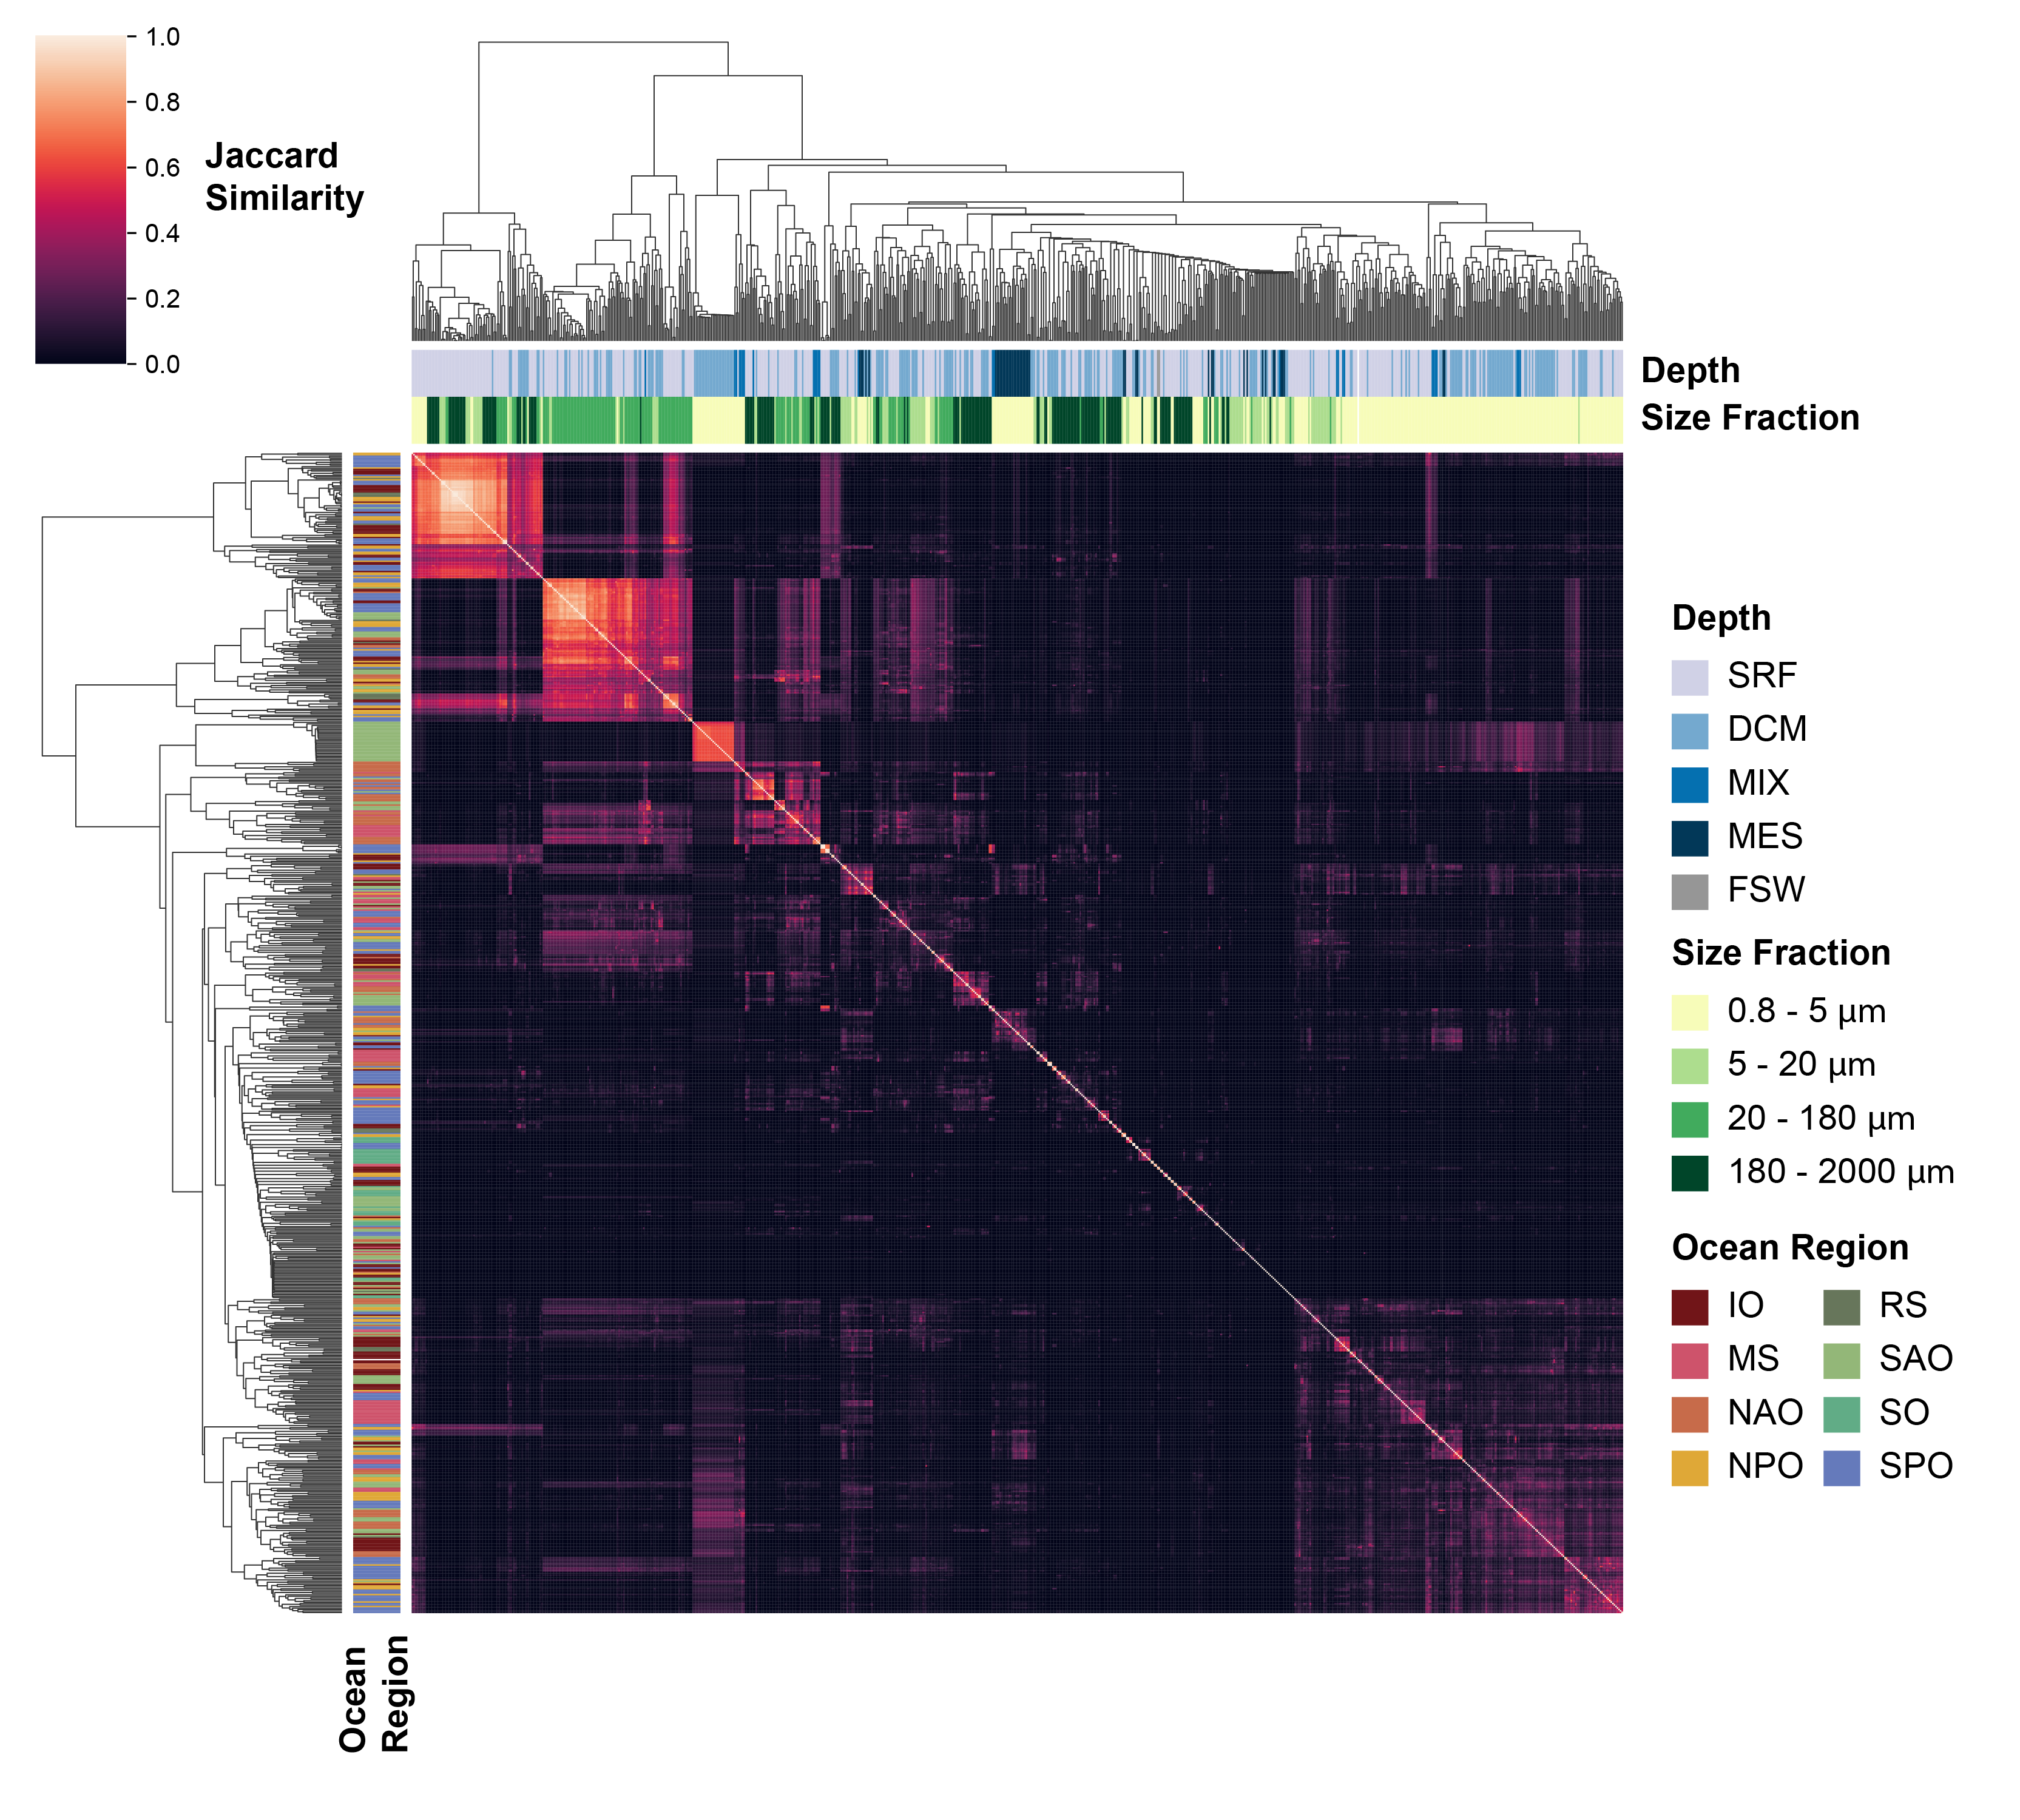
\includegraphics[width=0.95\columnwidth]{si-figures/modified-sourmash-region-size_depth-01.png}
    \caption{Sourmash comparison of all metagenomic samples from Tara large size fraction dataset. A minhash comparison was calculated using sourmash (k=31, scale=10,000) of the 824 metagenomic samples corresponding to the large size fraction metagenomic data from Tara (PRJEB4352). The relative sequence content similarity is shown as Jaccard similarity. Hierarchical clustering of samples based on sequence content is shown and sample identity (sample depth, size fraction, and ocean region) is highlighted by colored blocks.}
    \label{fig:sourmash}
\end{figure}


\begin{figure}
    \centering
    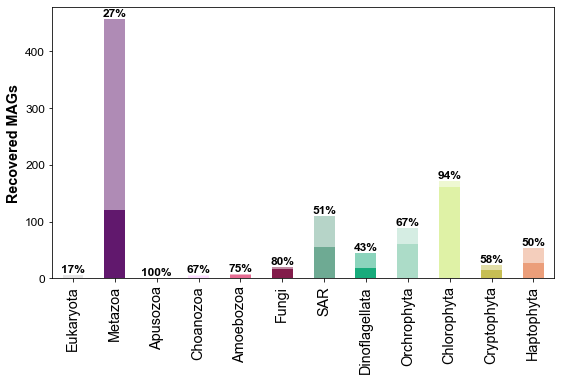
\includegraphics[width=0.9\columnwidth]{si-figures/MAGS_recovered.png}
    \caption{TOPAZ Recovered Eukaryotic MAGs. Course level taxonomic categorization of recovered eukaryotic TOPAZ MAGs (n=988). For each taxonomic group, the total number of MAGs is depicted. MAGs within a taxonomic group that were highly complete ($>30\%$ BUSCO completeness) are shaded and the percentage of highly complete MAGs for each taxonomic group is reported. }
    \label{fig:recovered}
\end{figure}

\begin{landscape}
\begin{figure}
    \centering
    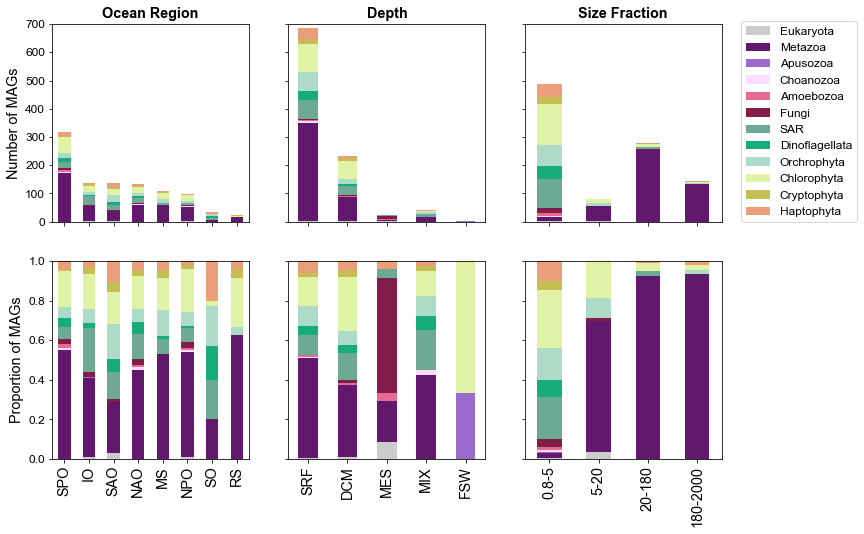
\includegraphics[width=0.95\columnwidth]{si-figures/ALL_MAG_distributions.png}
    \caption{TOPAZ Eukaryotic MAG as recovered by assembly group. The taxonomic breakdown of eukaryotic MAGs recovered within each general type of assembly group (based on Ocean Region, Depth, and Size Fraction) for all eukaryotic MAGs recovered in this study (n=988). Taxonomy is shown both as a total number recovered (top) and as a proportion of MAGs recovered for a given category (bottom). }
    \label{fig:all-dist}
\end{figure}
\end{landscape}

\begin{figure}
    \centering
    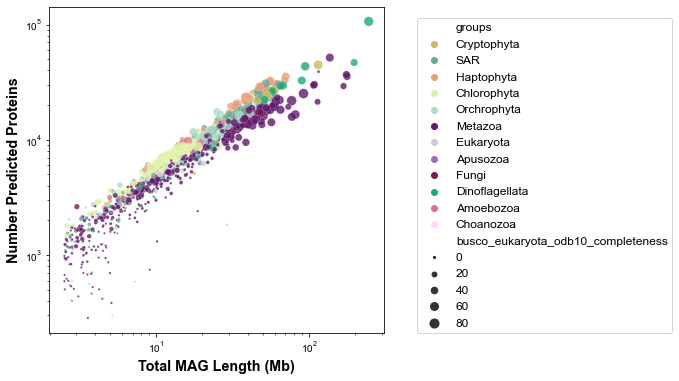
\includegraphics[width=0.95\columnwidth]{si-figures/ALL_MAGS_Num-Prot-Leng.png}
    \caption{The number of predicted proteins as a function of total MAG length.The number of predicted proteins for each eukaryotic TOPAZ mag (n=988) is plotted against the total MAG length (Mb). Each MAG is colored by its taxonomic group and the size of the circle is scaled by the estimated BUSCO completeness.}
    \label{fig:all-prot-len}
\end{figure}

\begin{landscape}
\begin{figure}
    \centering
    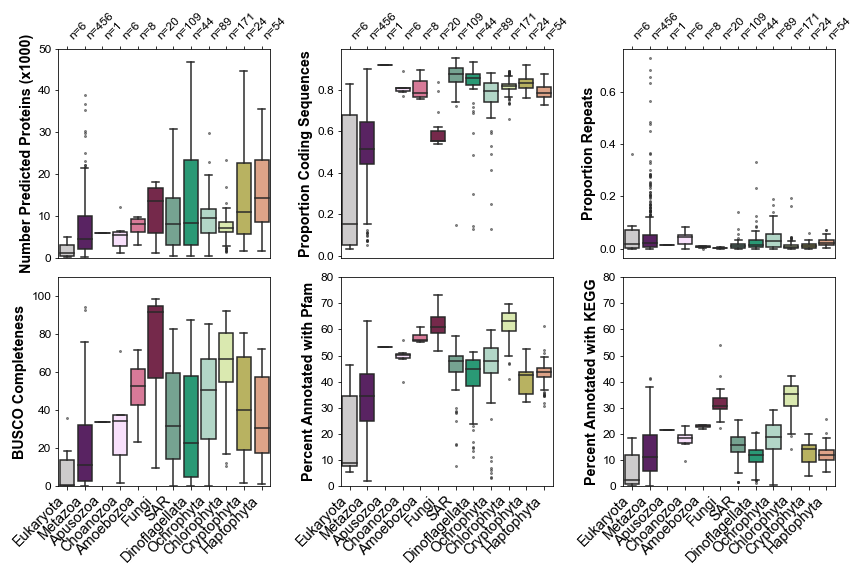
\includegraphics[width=0.9\columnwidth]{si-figures/ALL_MAG_protein_bar_plots.png}
    \caption{Genomic traits of recovered eukaryotic completeness, protein predictions, and annotation of all eukaryotic TOPAZ MAGs (n=988). The number of predicted proteins, proportion coding sequences, proportion repeat content, BUSCO completeness, percent annotation with Pfam and KEGG ontology are shown as box and whisker plots for the major higher-level groups that we define for this paper.}
    \label{fig:all-prot-bar}
\end{figure}
\end{landscape}

\begin{landscape}
\begin{figure}
    \centering
    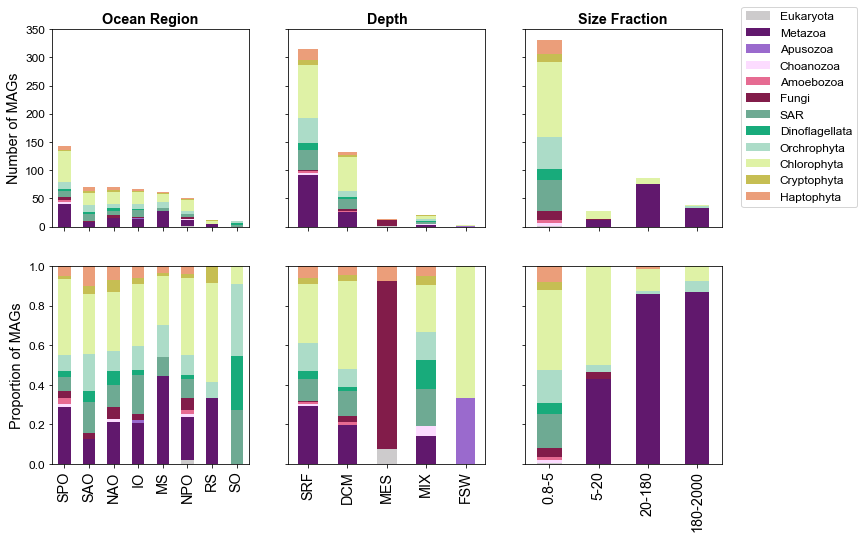
\includegraphics[width=0.95\columnwidth]{si-figures/HQ_MAG_distributions.png}
    \caption{TOPAZ Highly Complete Eukaryotic MAGs as recovered by assembly group. The taxonomic breakdown of eukaryotic MAGs recovered within each general type of assembly group (based on Ocean Region, Depth, and Size Fraction) for highly complete eukaryotic MAGs ($>30\%$ BUSCO completeness)recovered in this study (n=485)). Taxonomy is shown both as a total number recovered (top) and as a proportion of MAGs recovered for a given category (bottom). }
    \label{fig:hq-dist}
\end{figure}
\end{landscape}


\begin{landscape}
\begin{figure}
    \centering
    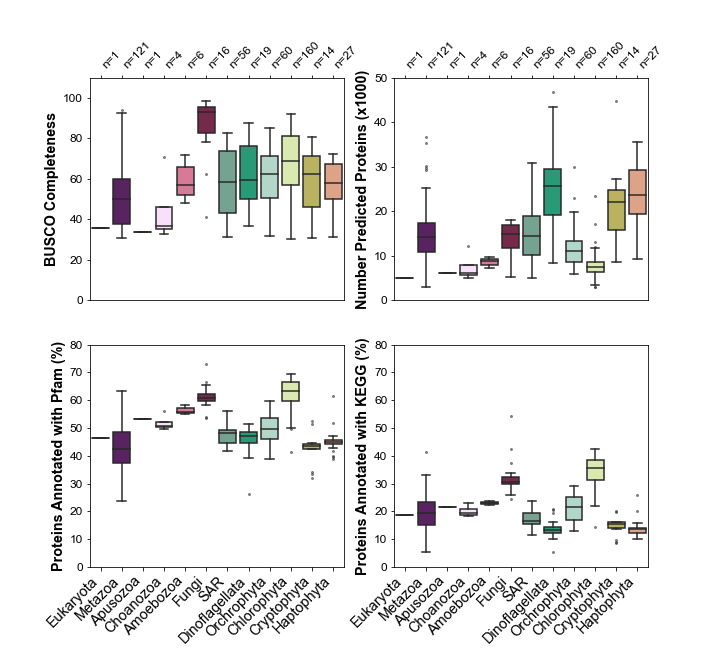
\includegraphics[width=0.9\columnwidth]{si-figures/HQ_MAG_protein_bar_plots.png}
    \caption{Genomic traits of recovered eukaryotic completeness, protein predictions, and annotation of the highly complete eukaryotic TOPAZ MAGs (n=485). The number of predicted proteins, proportion coding sequences, proportion repeat content, BUSCO completeness, percent annotation with Pfam and KEGG ontology are shown as box and whisker plots for the major higher-level groups that we define for this paper.}
    \label{fig:hq-prot-bar}
\end{figure}
\end{landscape}


\begin{figure}
    \centering
    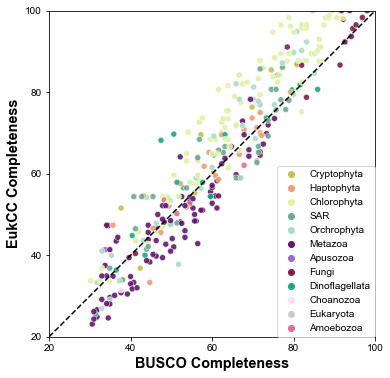
\includegraphics[width=0.8\columnwidth]{si-figures/HQ_BUSCO-EukCC-comp.png}
    \caption{A comparison of two metrics of eukaryotic completeness. BUSCO completeness as defined based on the presence and absence of genes within the eukaryota\_odb10 dataset was compared against the estimated EukCC completeness based on estimated lineages of given MAGs. Generally, it was observed that EukCC performed particualrly well for certain groups (e.g. chlorophytes and fungi) and less well for others (e.g. metazoa).}
    \label{fig:eukcc}
\end{figure}


\begin{landscape}
\begin{figure}
    \centering
    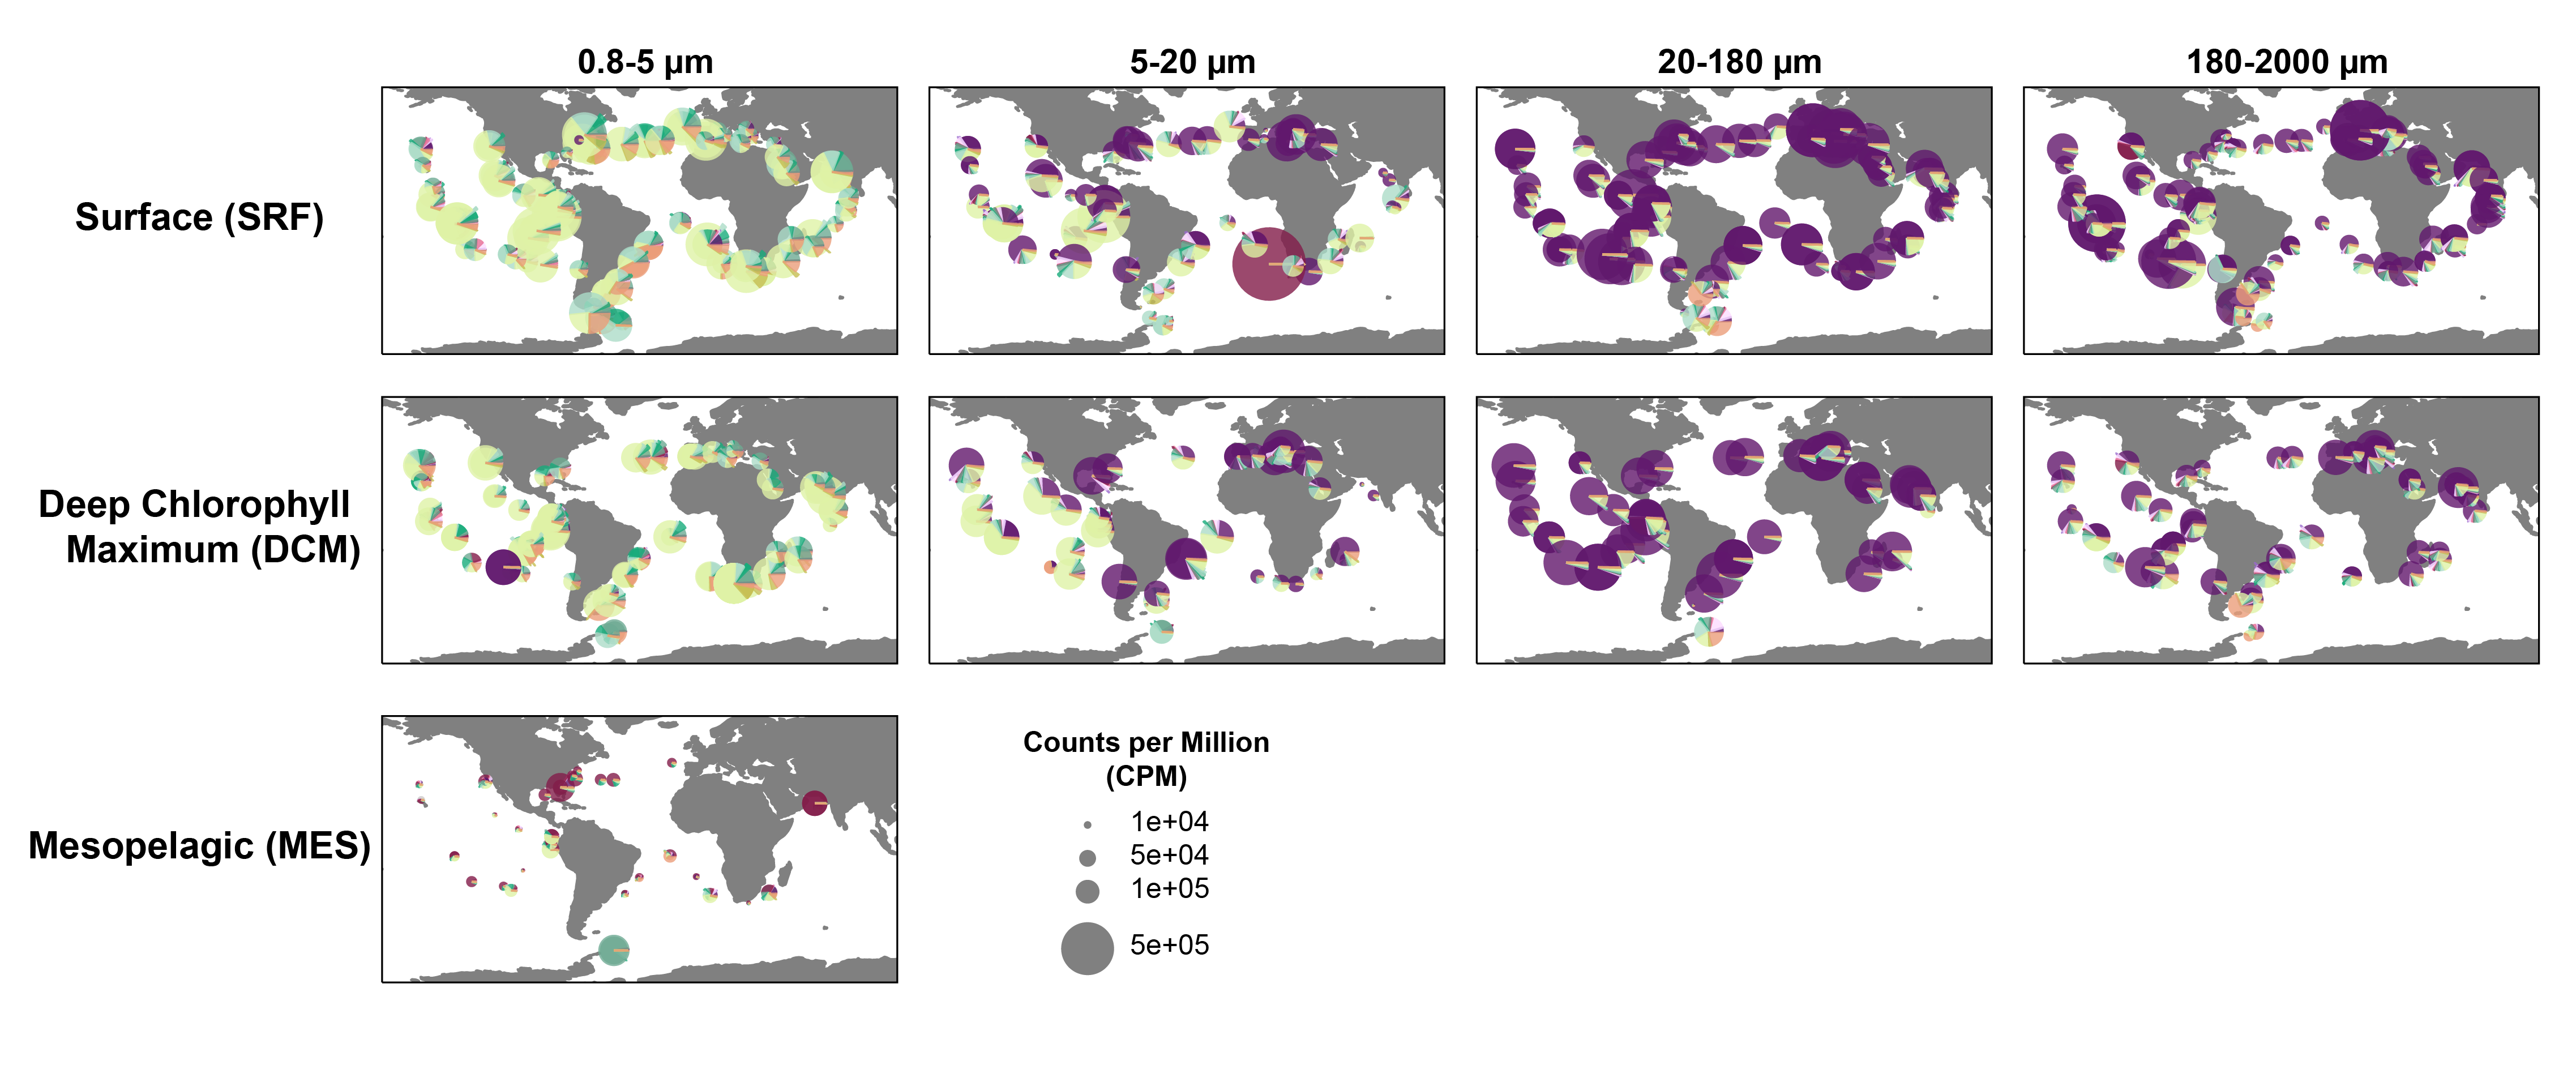
\includegraphics[width=0.95\columnwidth]{si-figures/Distribution-Map-Taxonomy-01.png}
    \caption{The distribution of the major lineages of eukaryotic TOPAZ MAGs recovered across the Tara metagenomic datasets. The counts per million (CPM) is depicted for all stations depicted by depth and size fraction.  }
    \label{fig:map}
\end{figure}
\end{landscape}

\begin{figure}
    \centering
    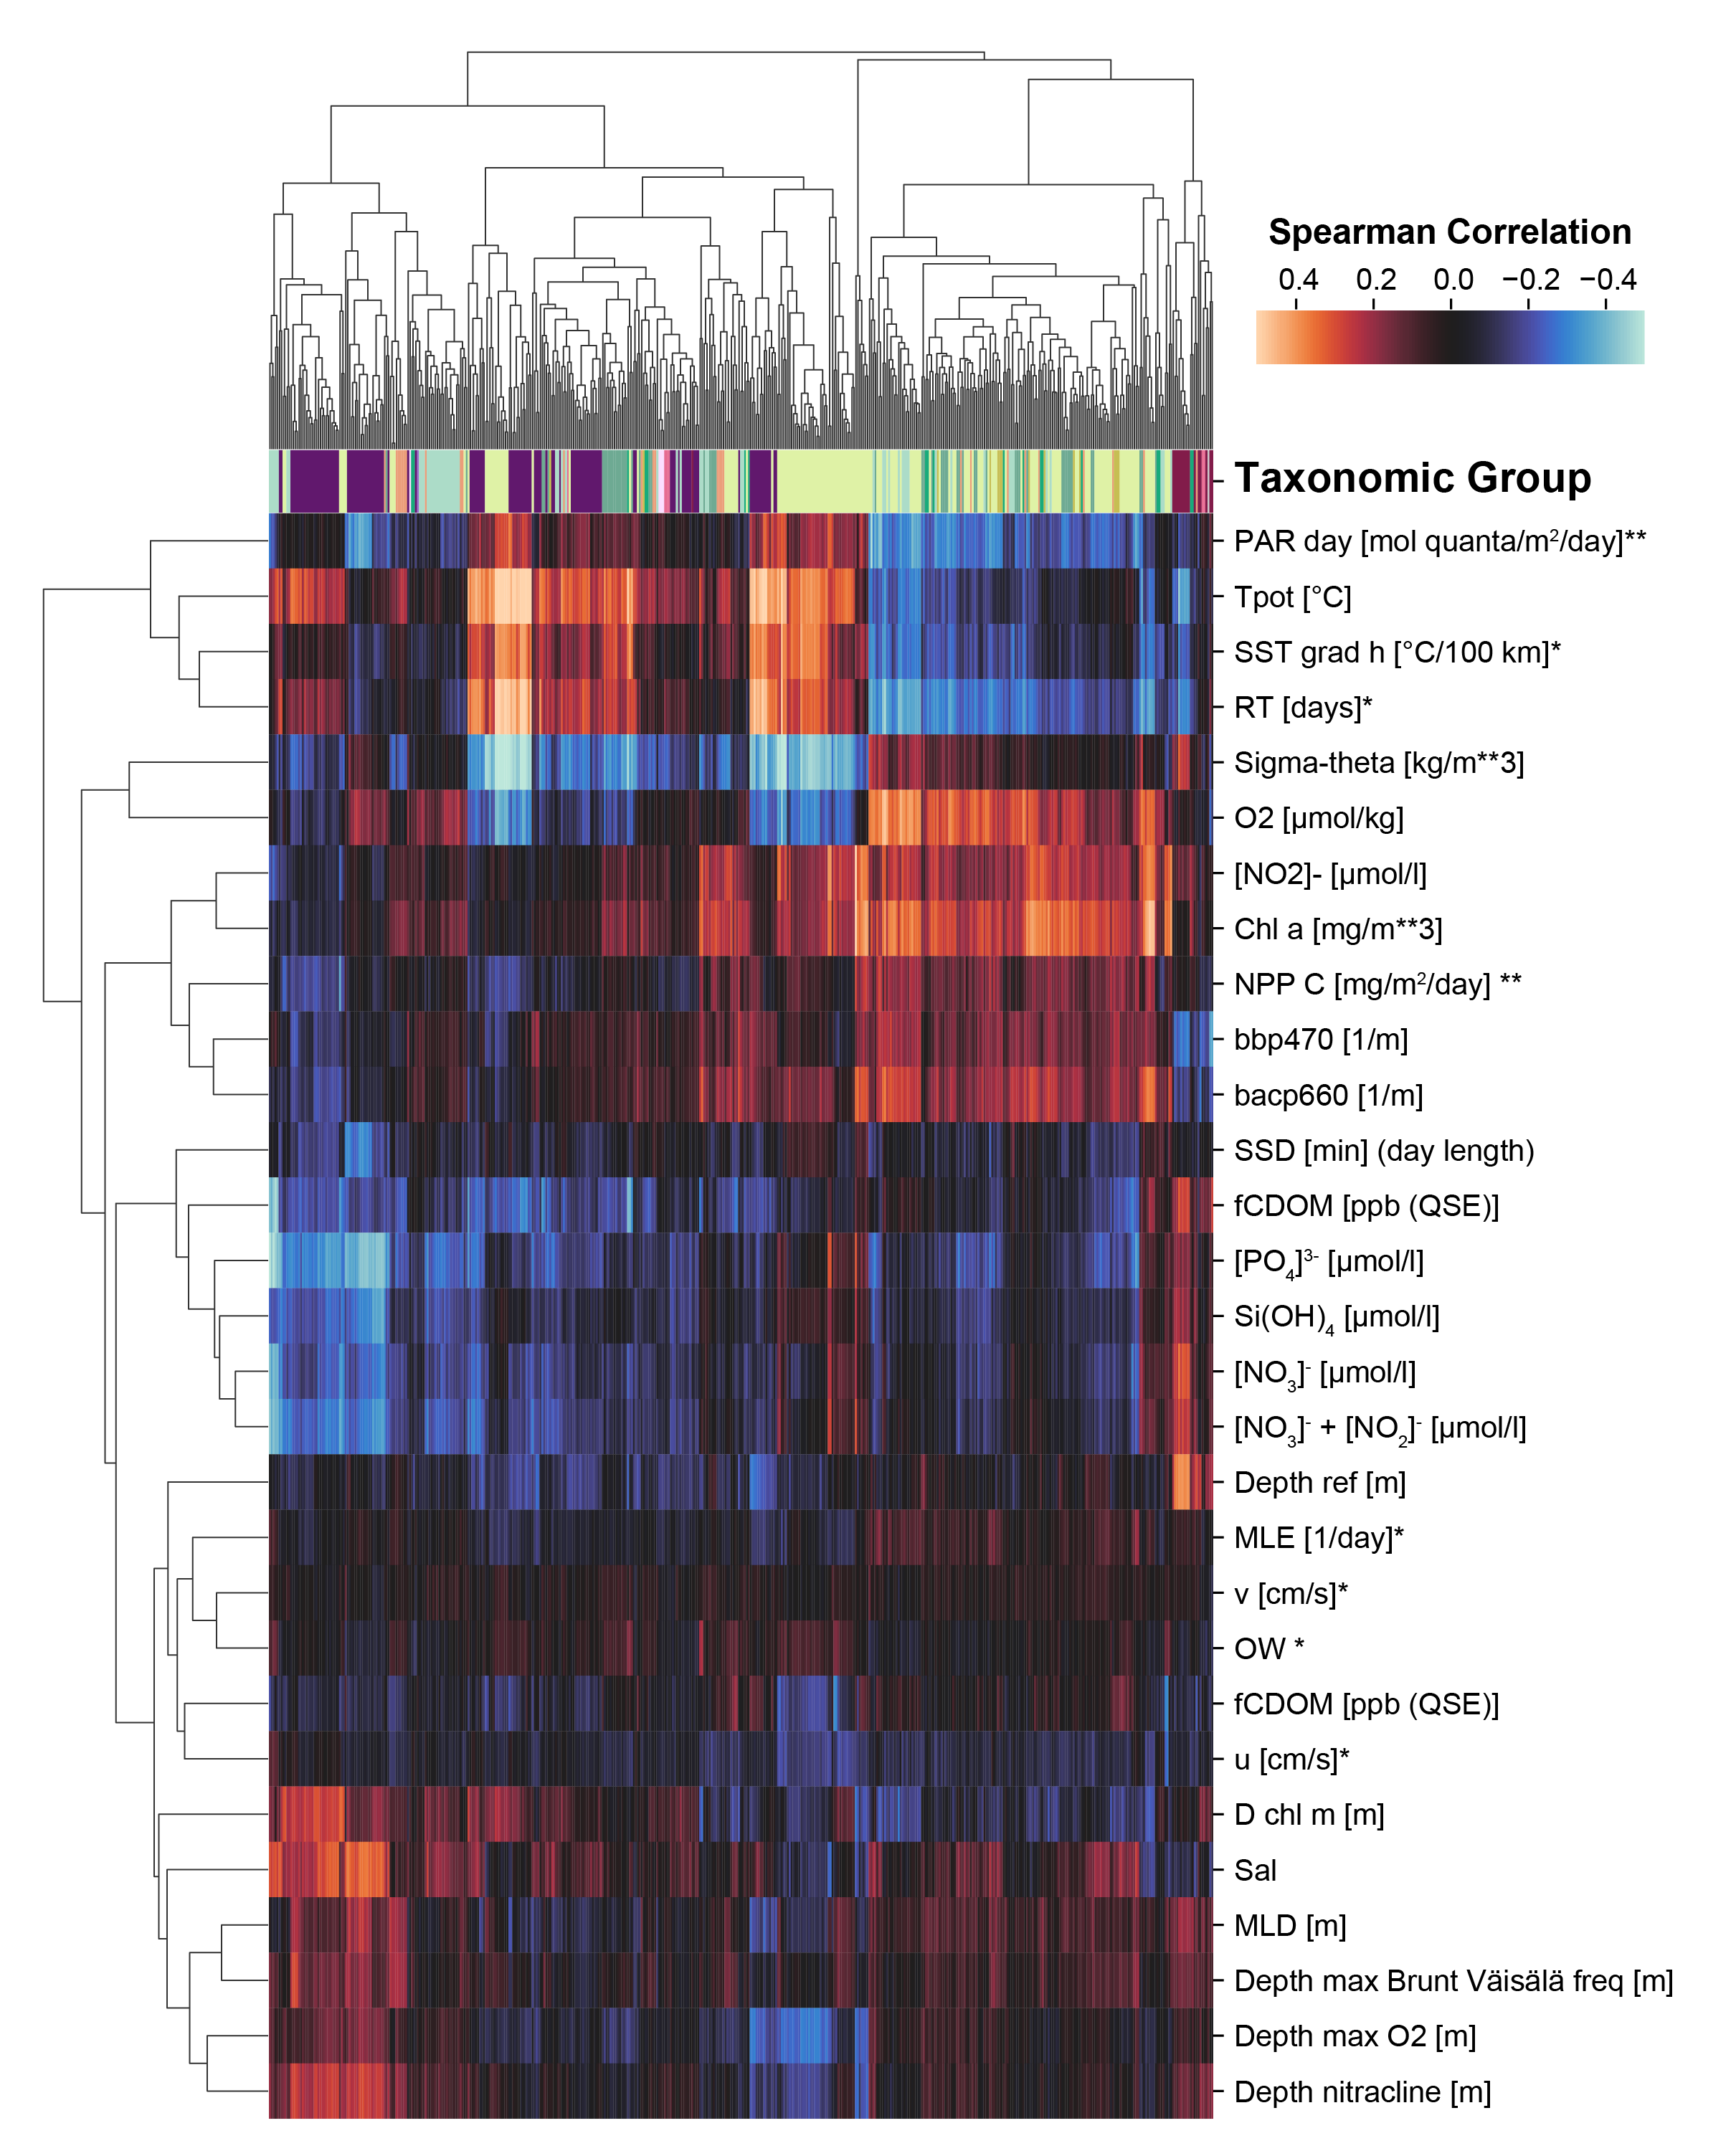
\includegraphics[width=0.9\columnwidth]{si-figures/modified-individual-mag-group-correlation-01.png}
    \caption{ }
    \label{fig:ind-corr}
\end{figure}


\begin{figure}
    \centering
    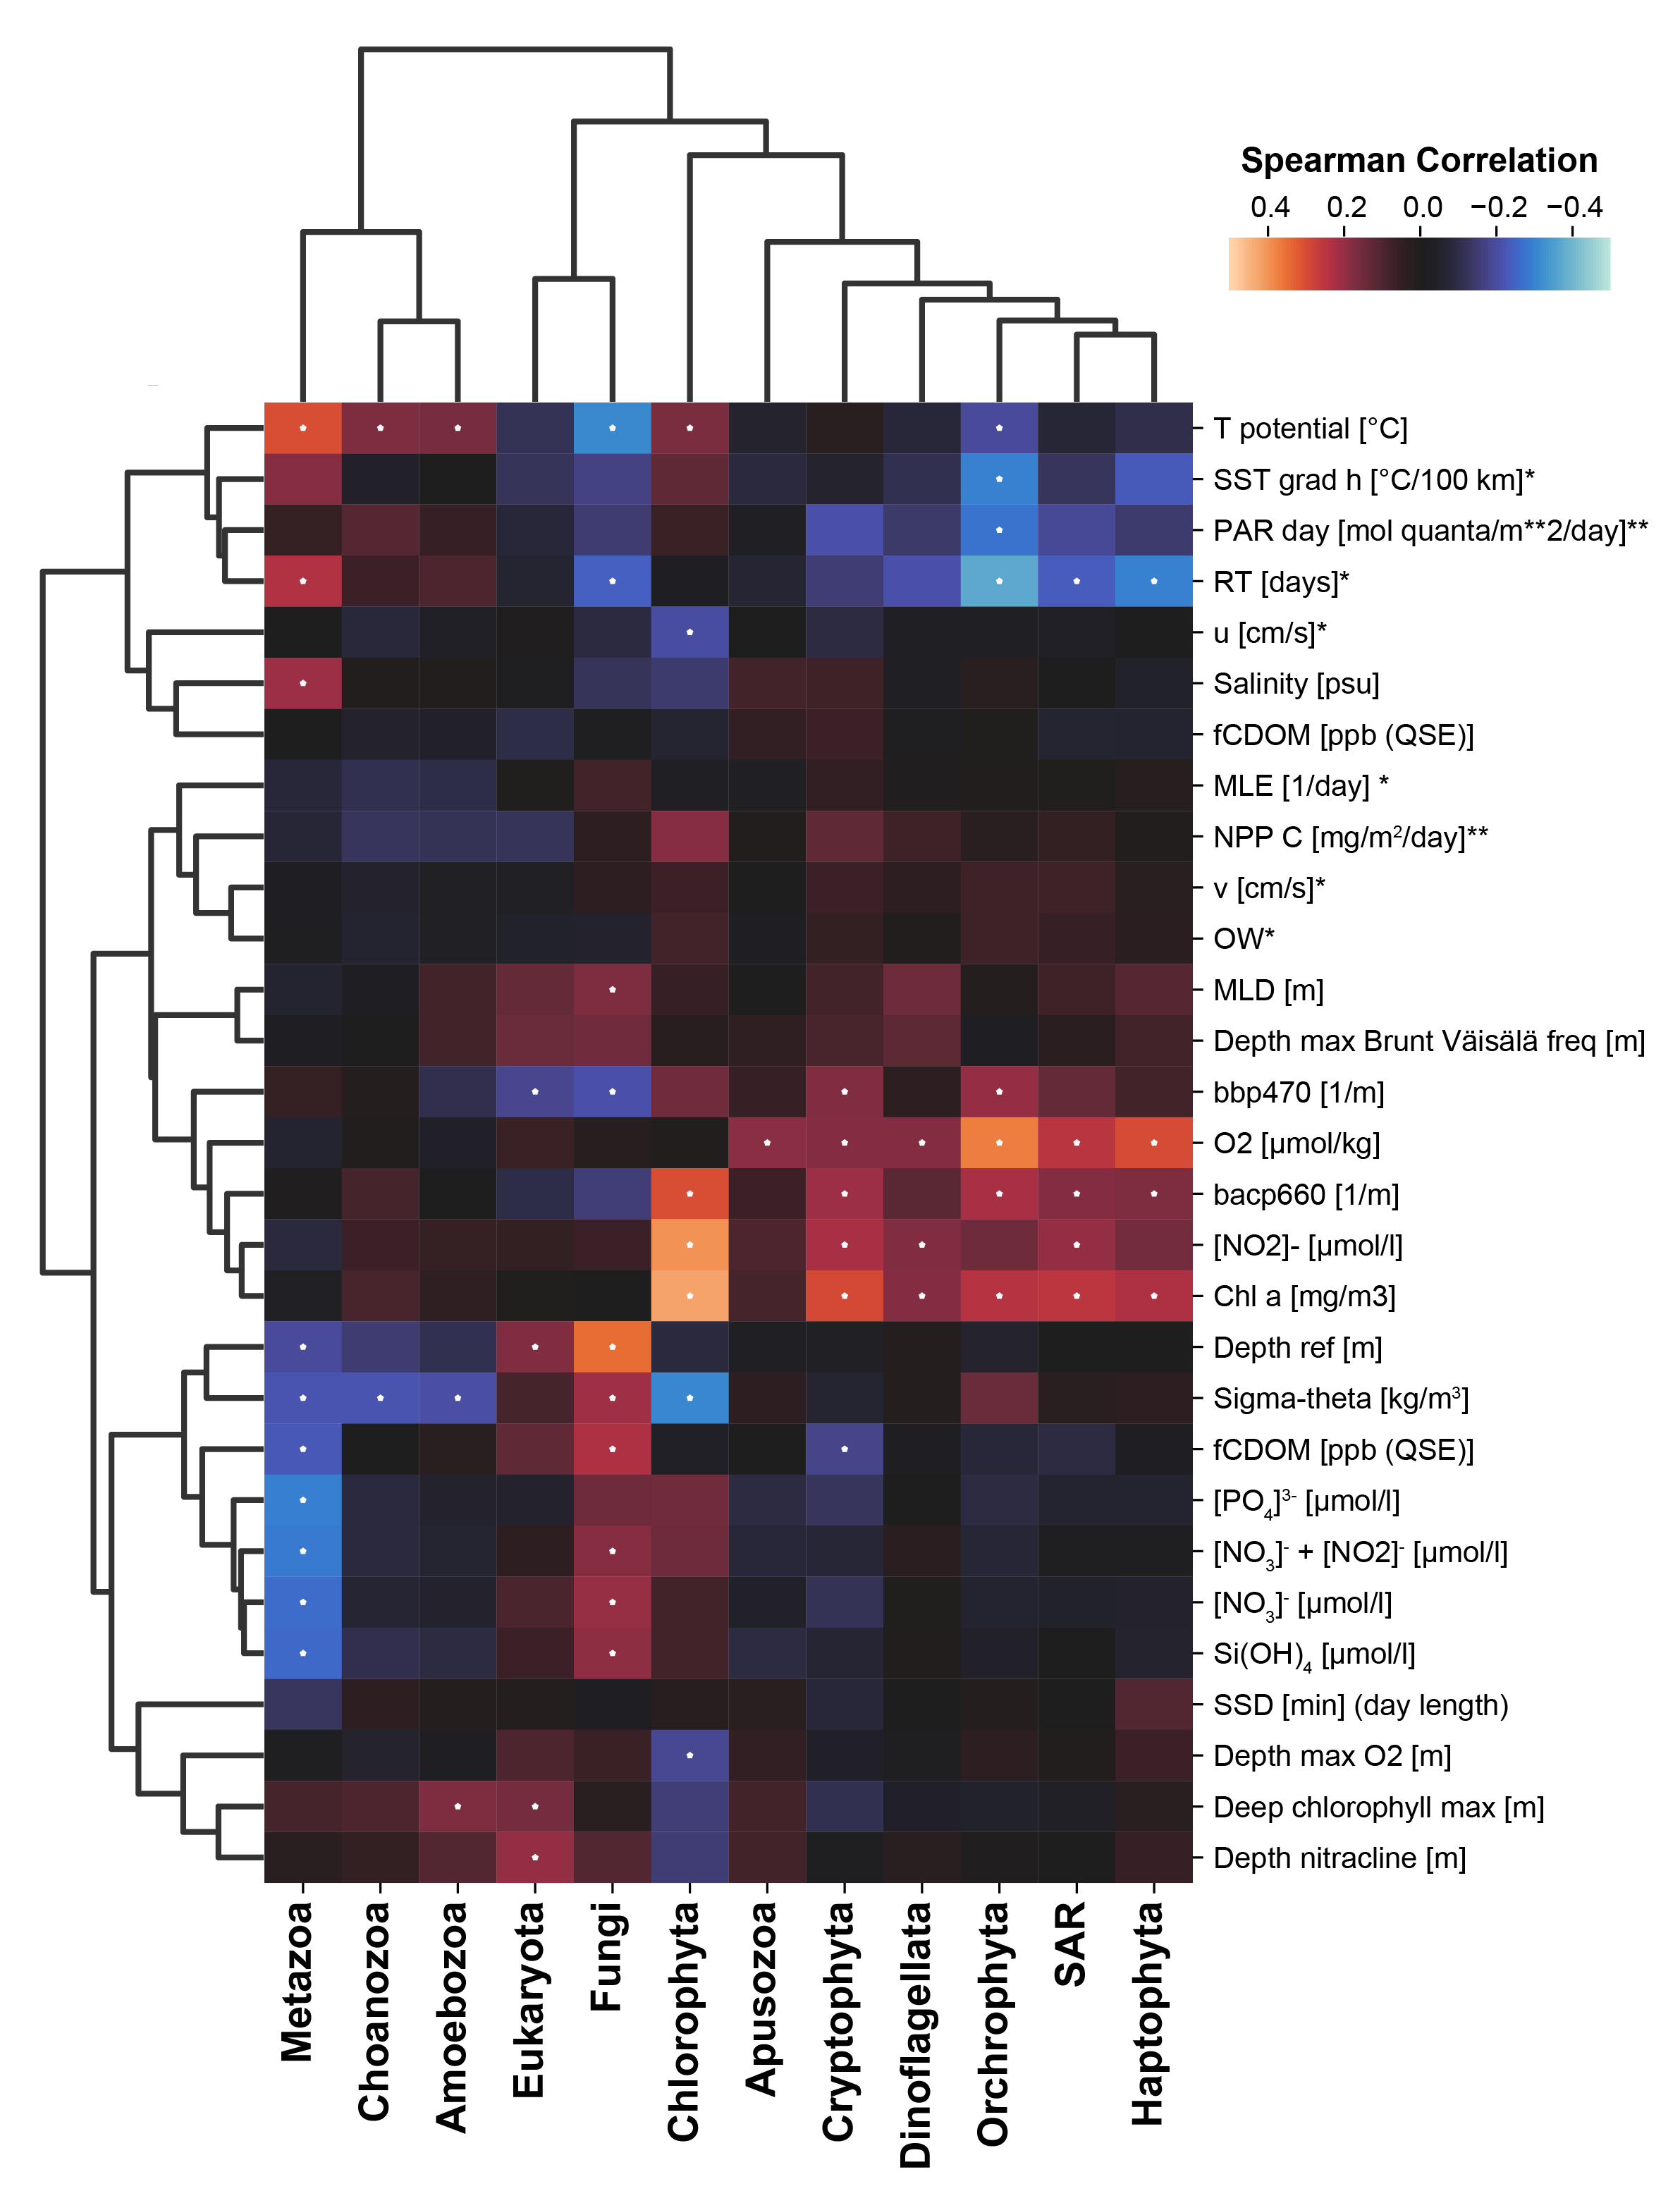
\includegraphics[width=0.9\columnwidth]{si-figures/mag-group-correlation-01.png}
    \caption{ }
    \label{fig:env-corr}
\end{figure}

\begin{figure}
    \centering
    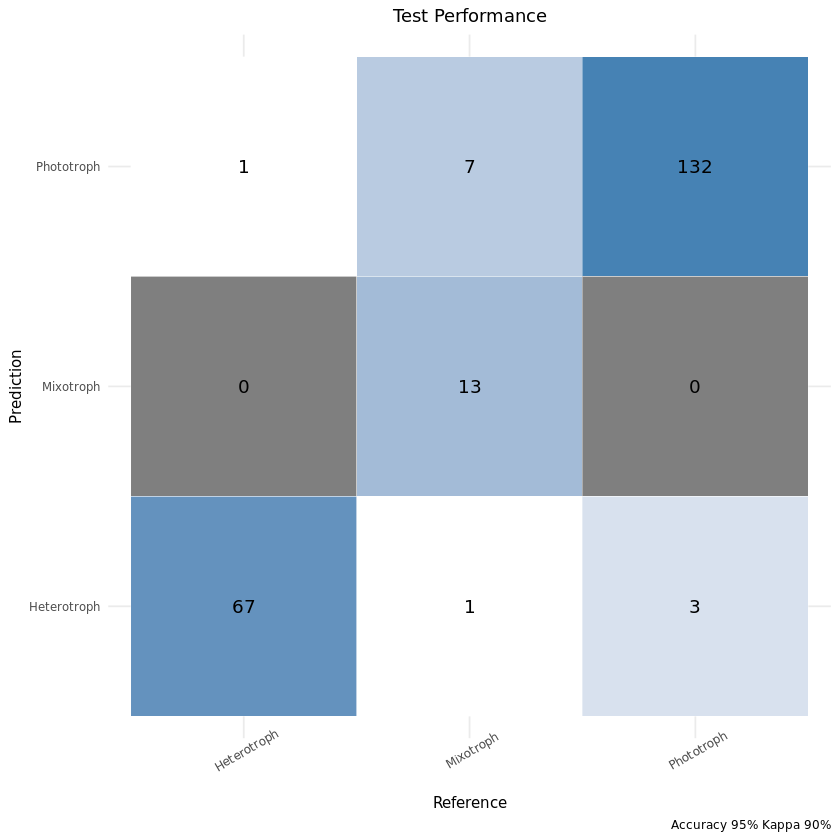
\includegraphics[width=0.95\columnwidth]{si-figures/confusionmatrix.png}
    \caption{}
    \label{fig:confusionmatrix}
\end{figure}

\begin{landscape}
    \begin{figure}
    \centering
    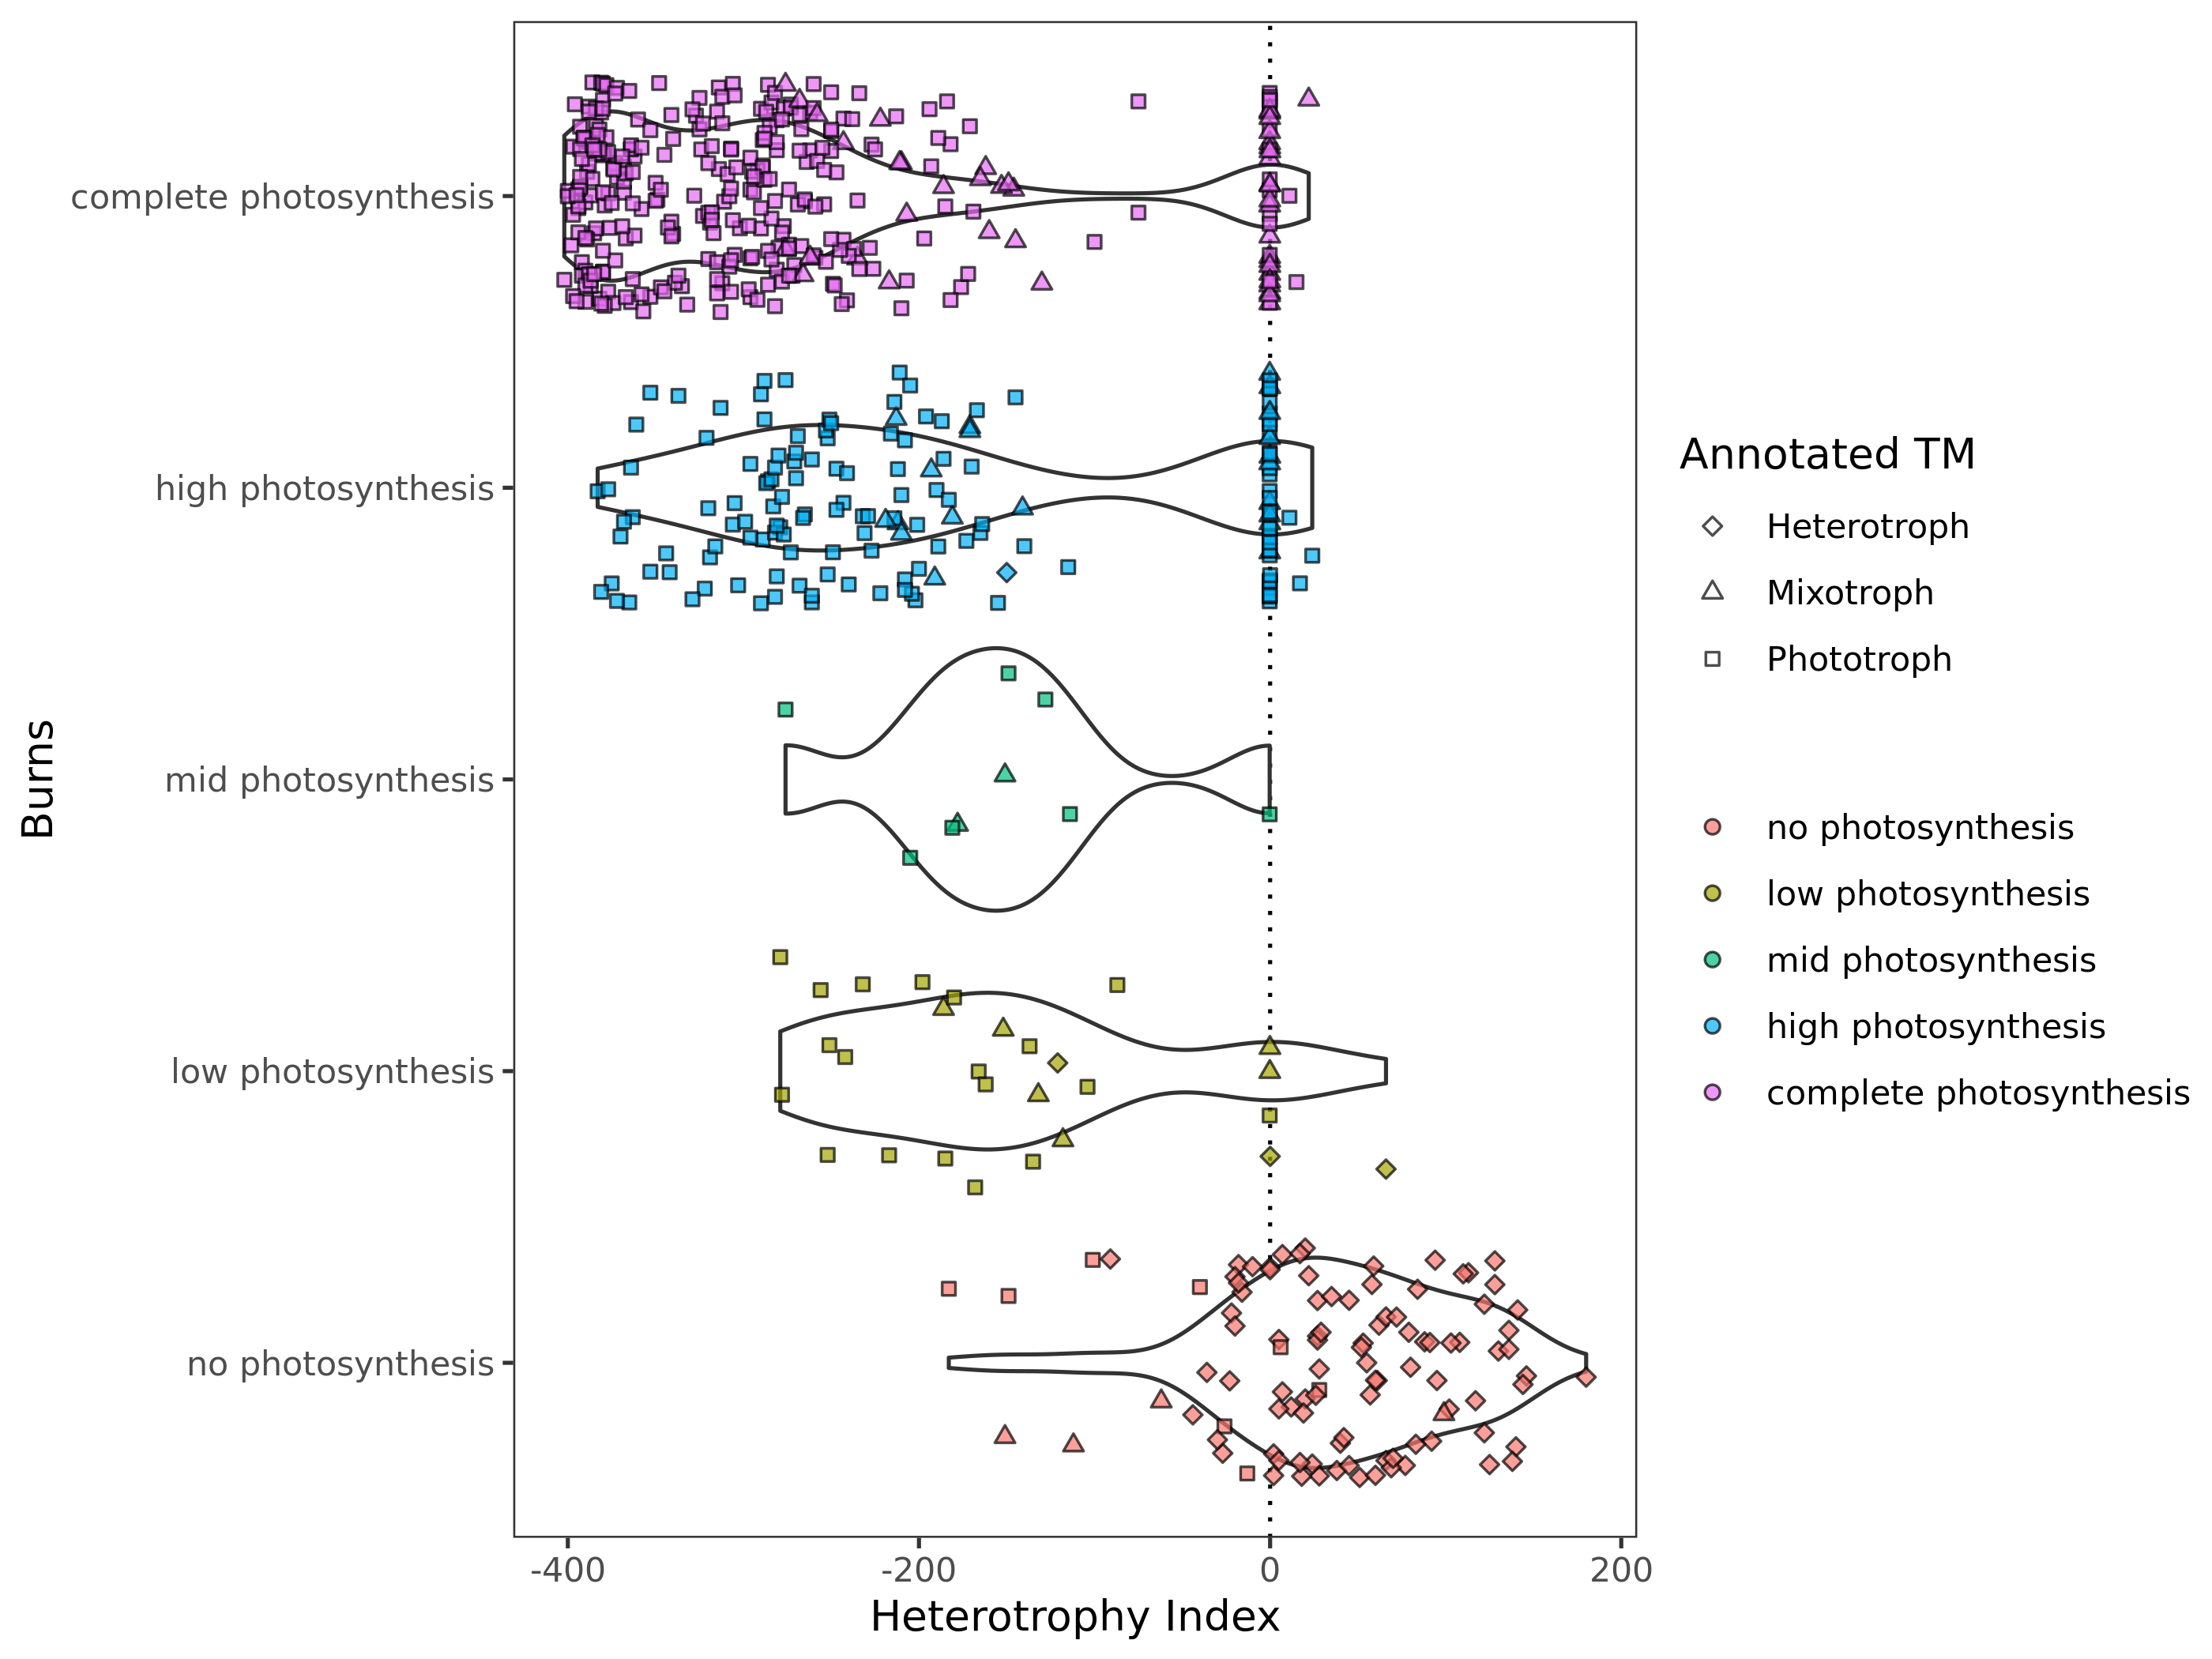
\includegraphics[width=0.95\columnwidth]{si-figures/burns_categories.png}
    \caption{}
    \label{fig:burns-cats}
\end{figure}
\end{landscape}


\begin{landscape}
\begin{figure}
    \centering
    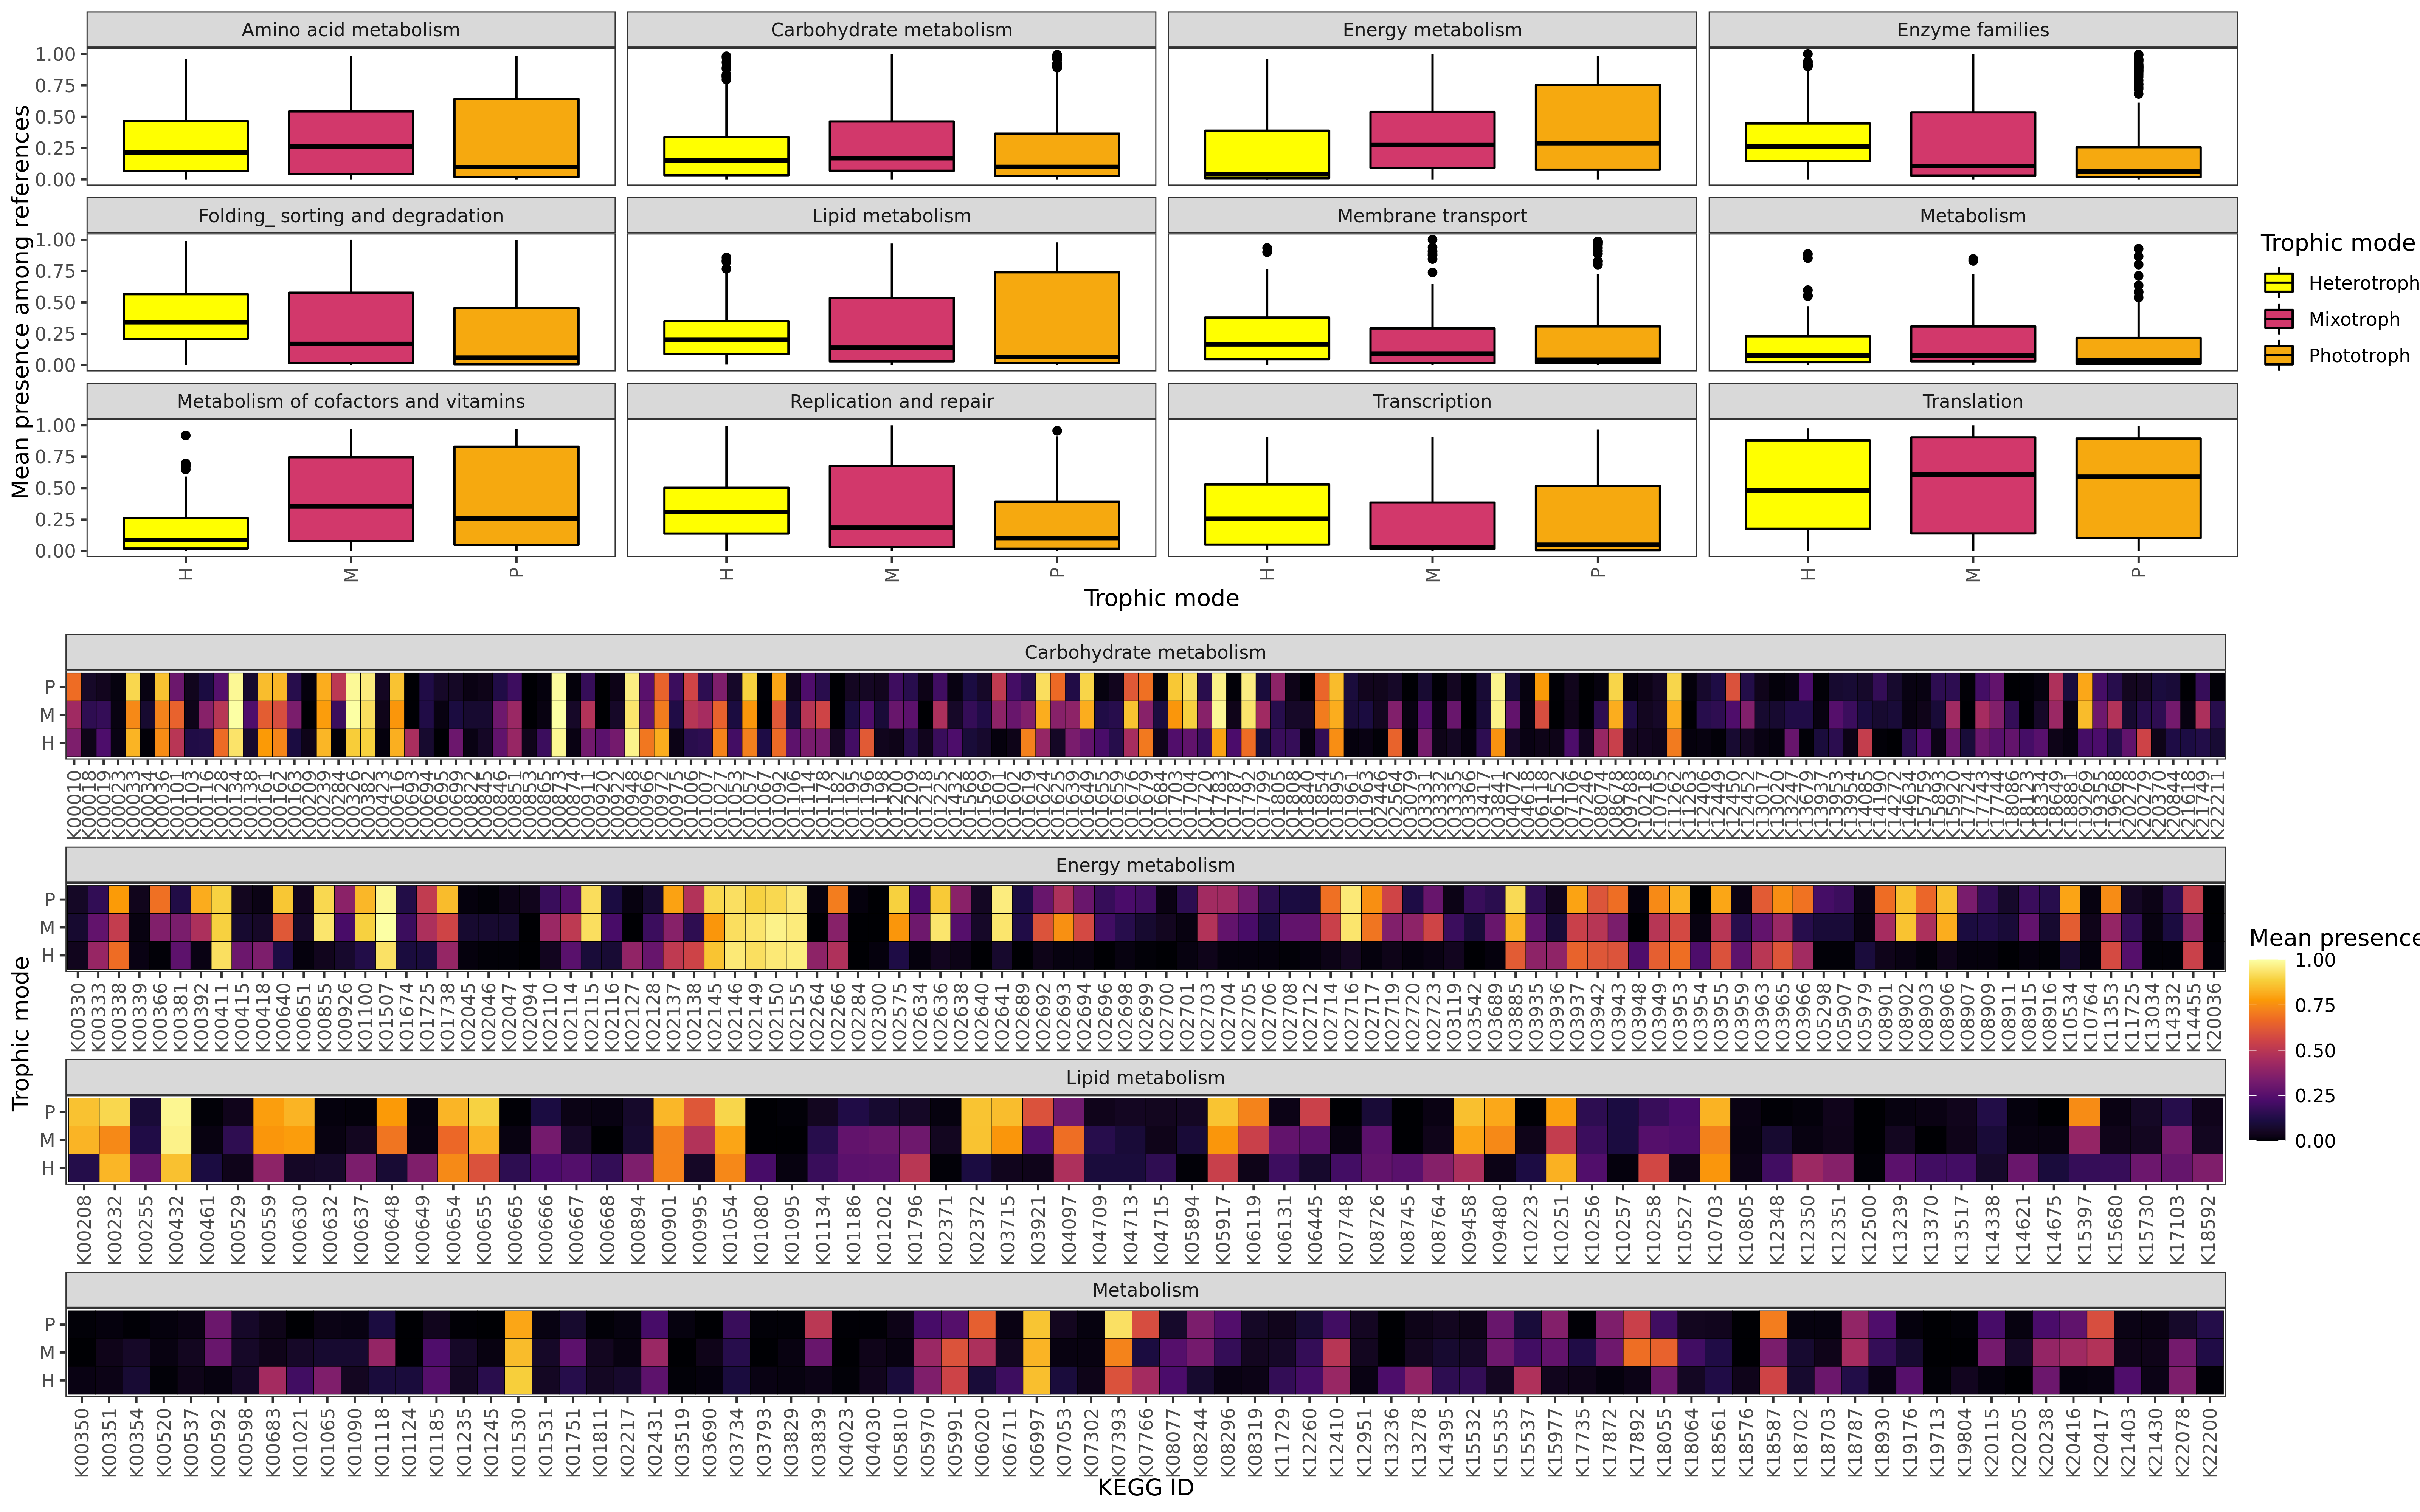
\includegraphics[width=0.95\columnwidth]{si-figures/KO_figure_trophy.png}
    \caption{Presence-absence of KEGG IDs as aggregated across all reference transcriptomes (MMETSP and EukProt) used in the trophic mode modeling process. The top boxplot panel shows the mean presence of the KEGG IDs implicated in the listed pathways for each of the three identified trophic modes, while the bottom heatmap panel shows the average presence of each individual KO along the horizontal axis for reference transcriptomes annotated as each major trophic mode (vertical axis).}
    \label{fig:ko-trophy}
\end{figure}
\end{landscape}

\begin{figure}
    \centering
    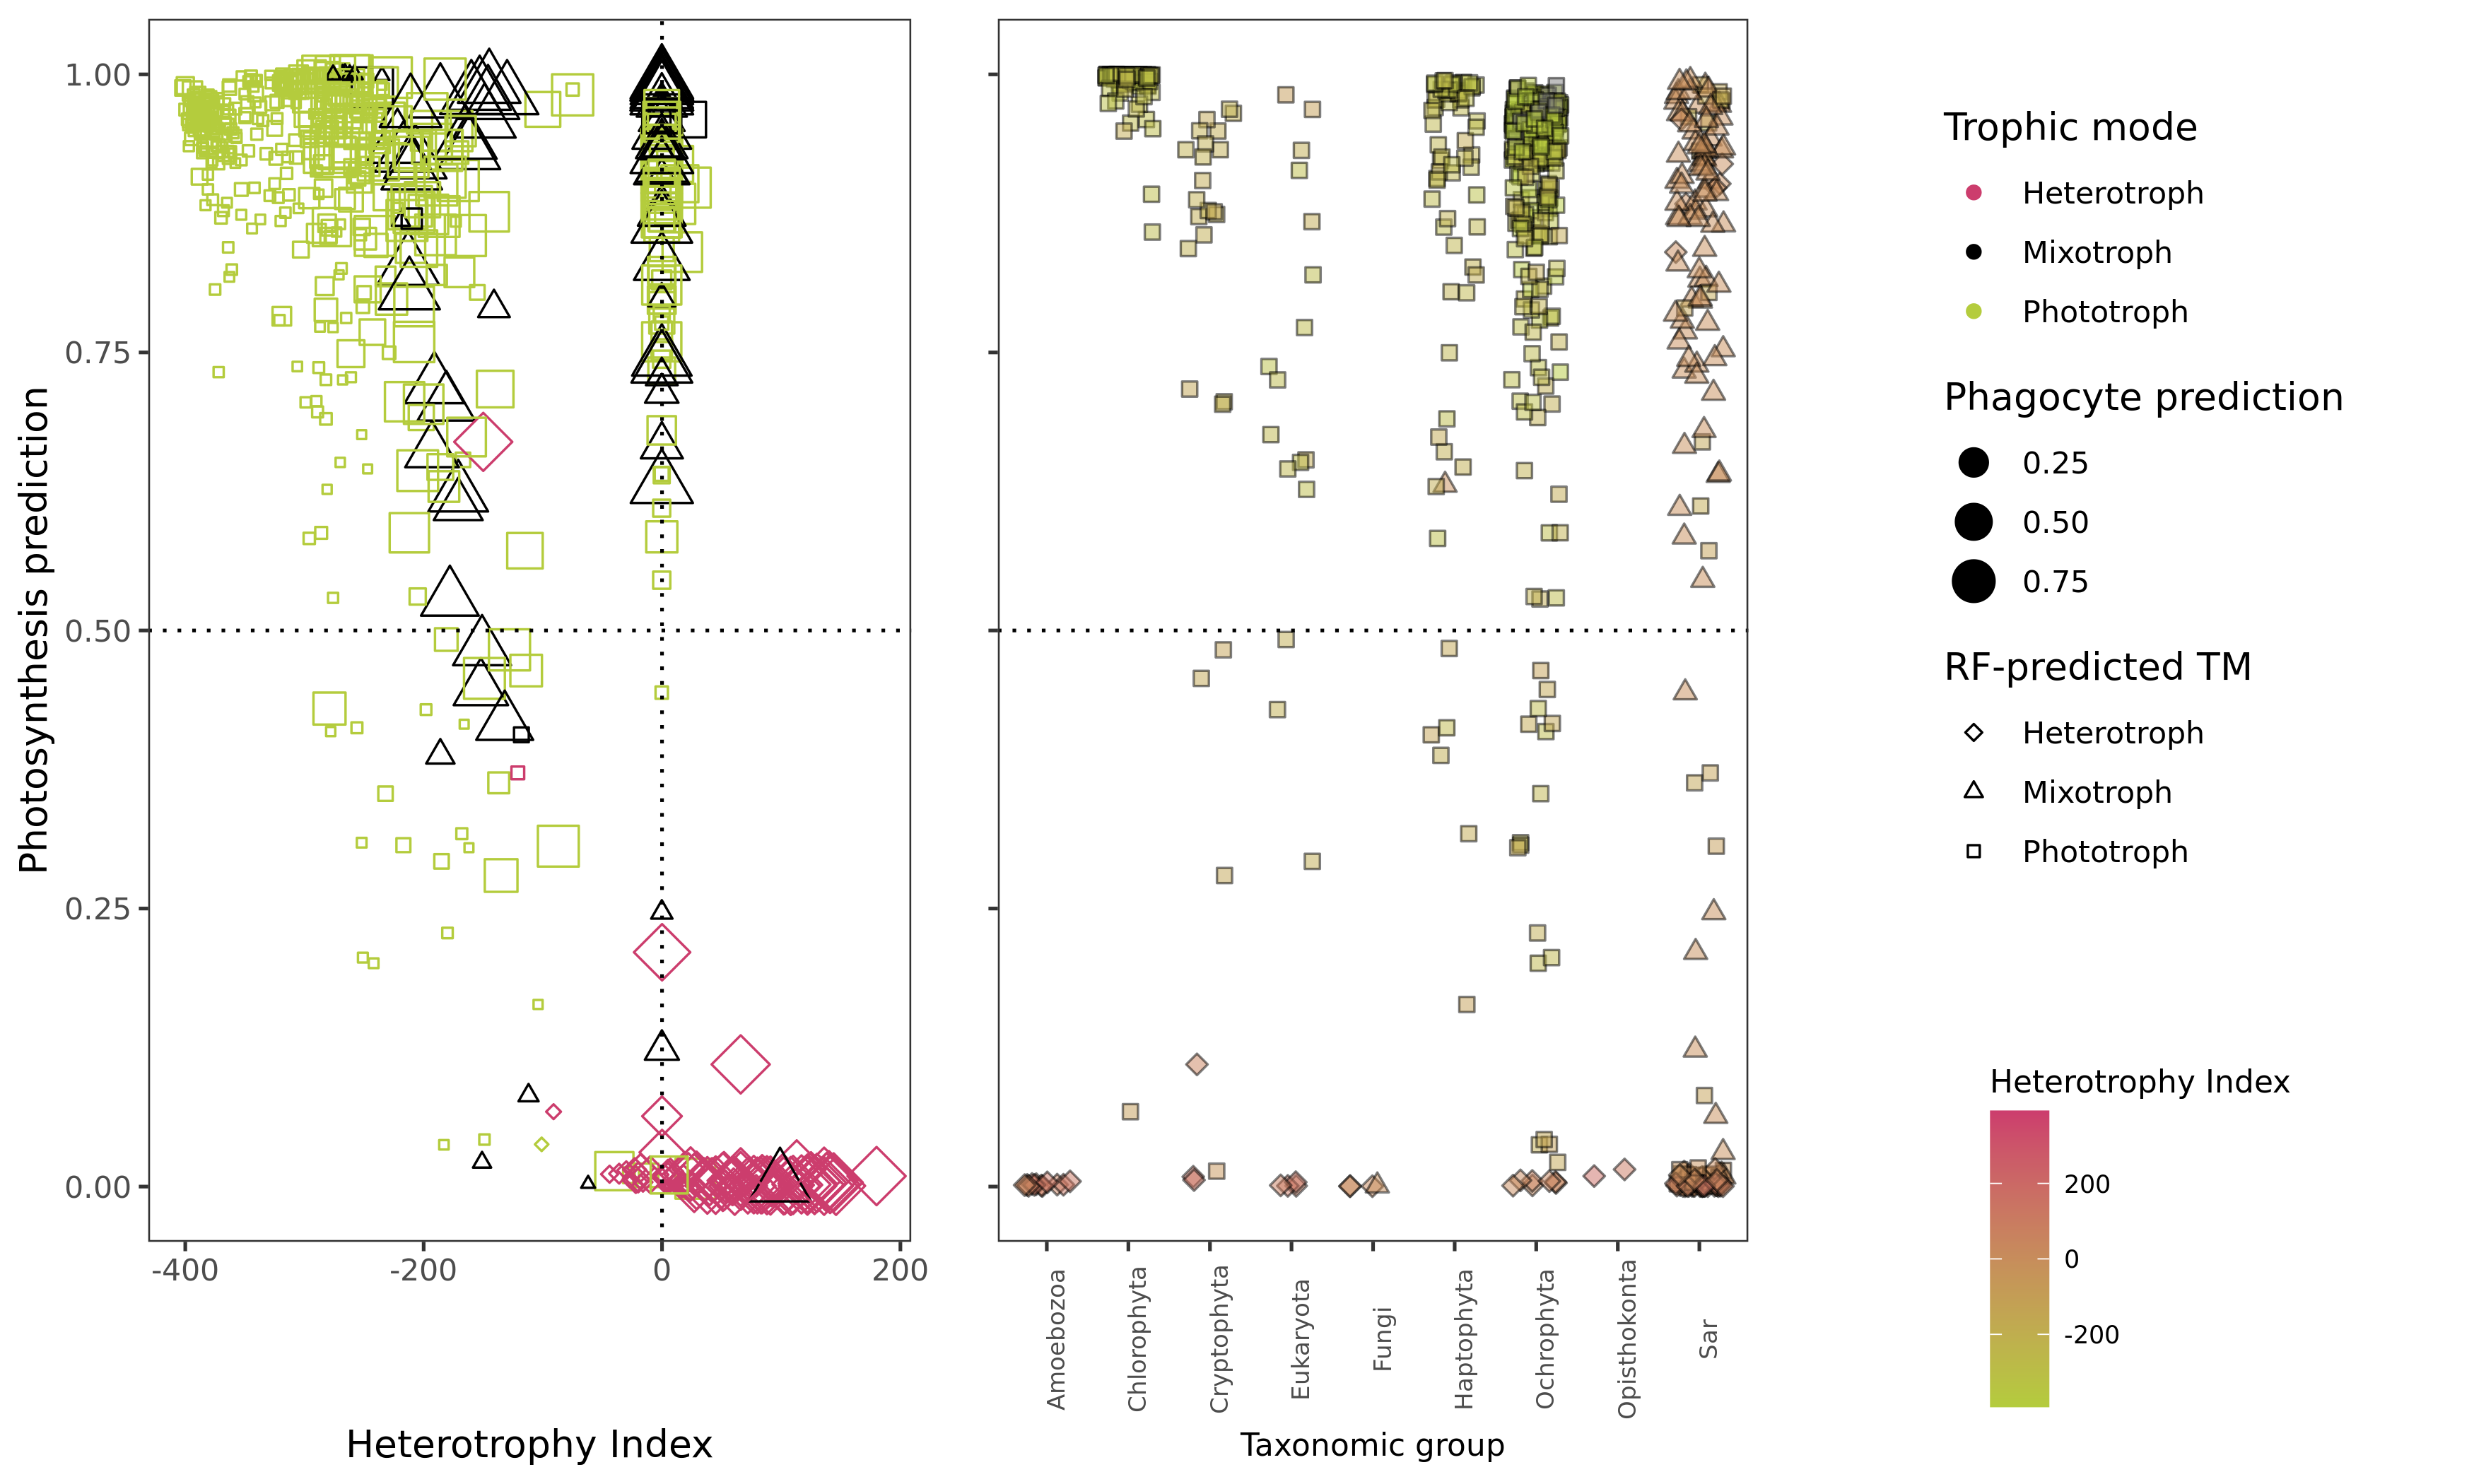
\includegraphics[width=0.95\columnwidth]{si-figures/mmetsp_burns.png}
    \caption{Comparison of the Burns \cite{burns2018gene} model to our Random Forest predictions and heterotrophy index calculations for the reference MMETSP transcriptomes. Left: Burns \cite{burns2018gene} photosynthesis predictions vs. composite heterotrophy index, scaled by the phagocytosis prediction and colored by the manually-annotated trophic mode. Right: predicted photosynthetic ability by taxonomic grouping, colored by the calculated heterotrophy index.}
    \label{fig:mmetsp-burns}
\end{figure}

\begin{figure}
    \centering
    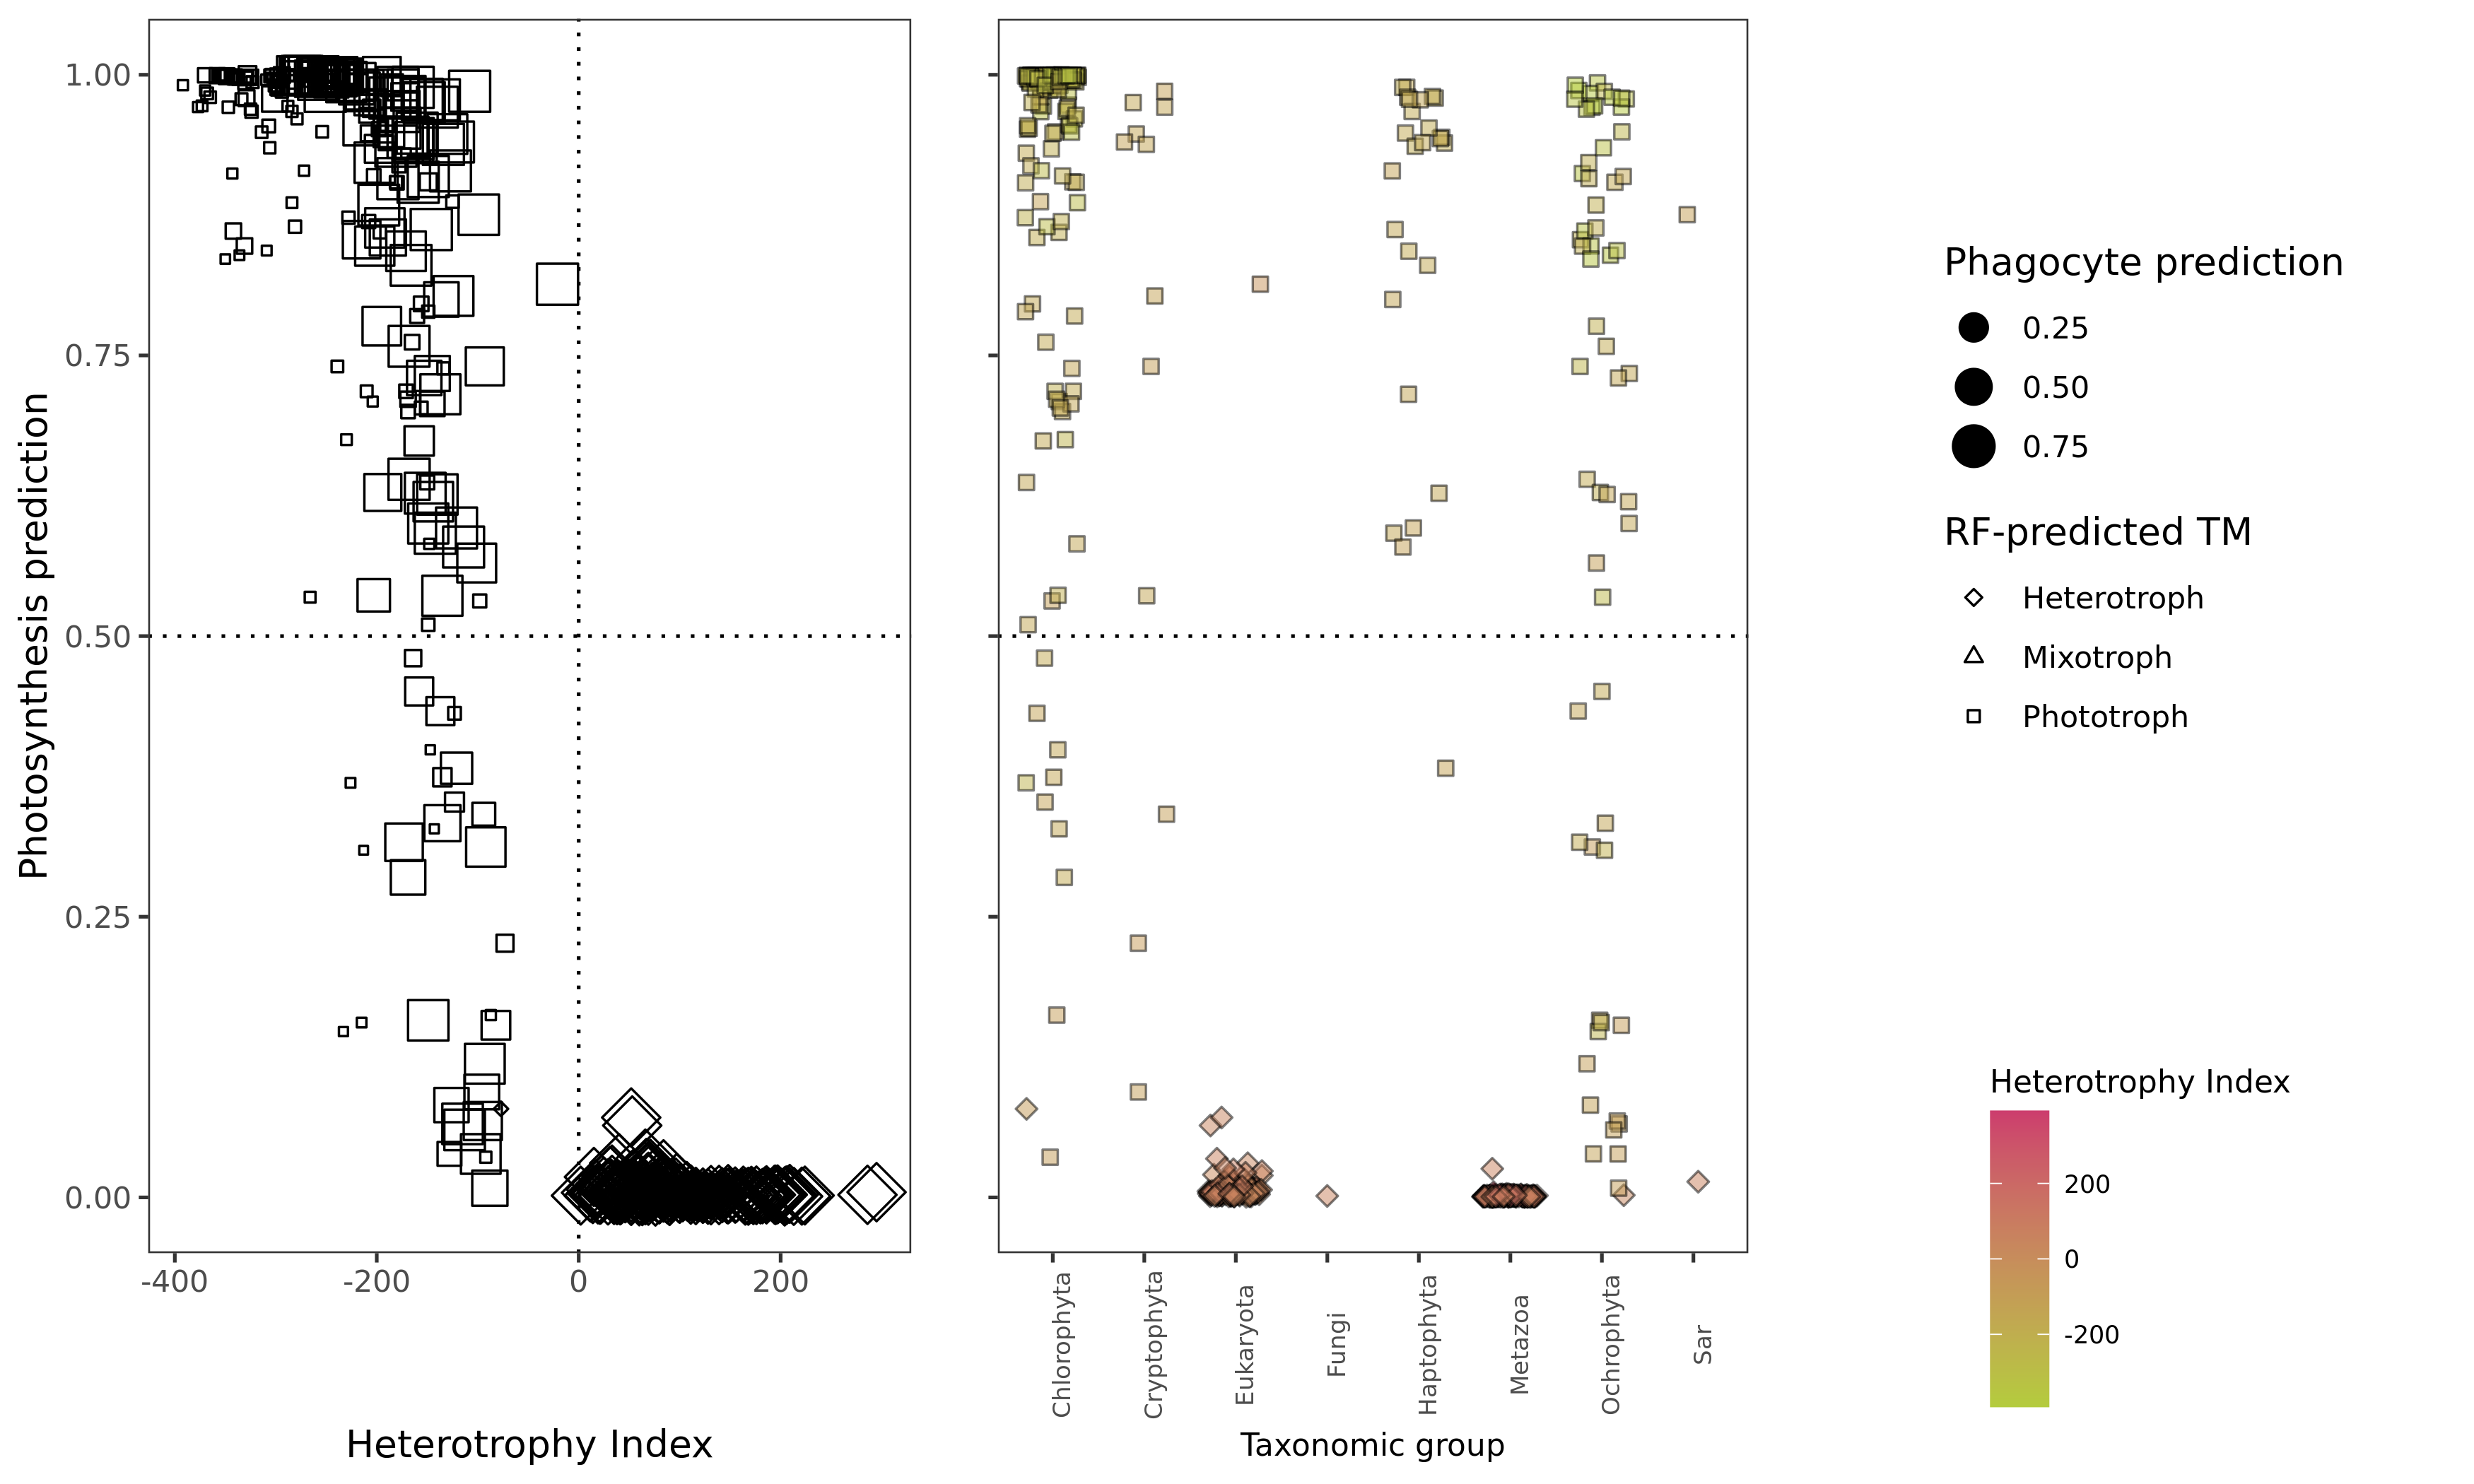
\includegraphics[width=0.95\columnwidth]{si-figures/mag_burns.png}
    \caption{Comparison of the Burns \cite{burns2018gene} model to our Random Forest predictions and heterotrophy index calculations for the TOPAZ MAGs. Left: Burns \cite{burns2018gene} photosynthesis predictions vs. composite heterotrophy index, scaled by the phagocytosis prediction and shape indicating the Random Forest-derived predicted trophic mode (note there is no color because trophic mode could not be manually annotated). Right: predicted photosynthetic ability by taxonomic grouping, colored by the calculated heterotrophy index.}
    \label{fig:mag-burns}
\end{figure}

\begin{landscape}
    \begin{figure}
        \centering
        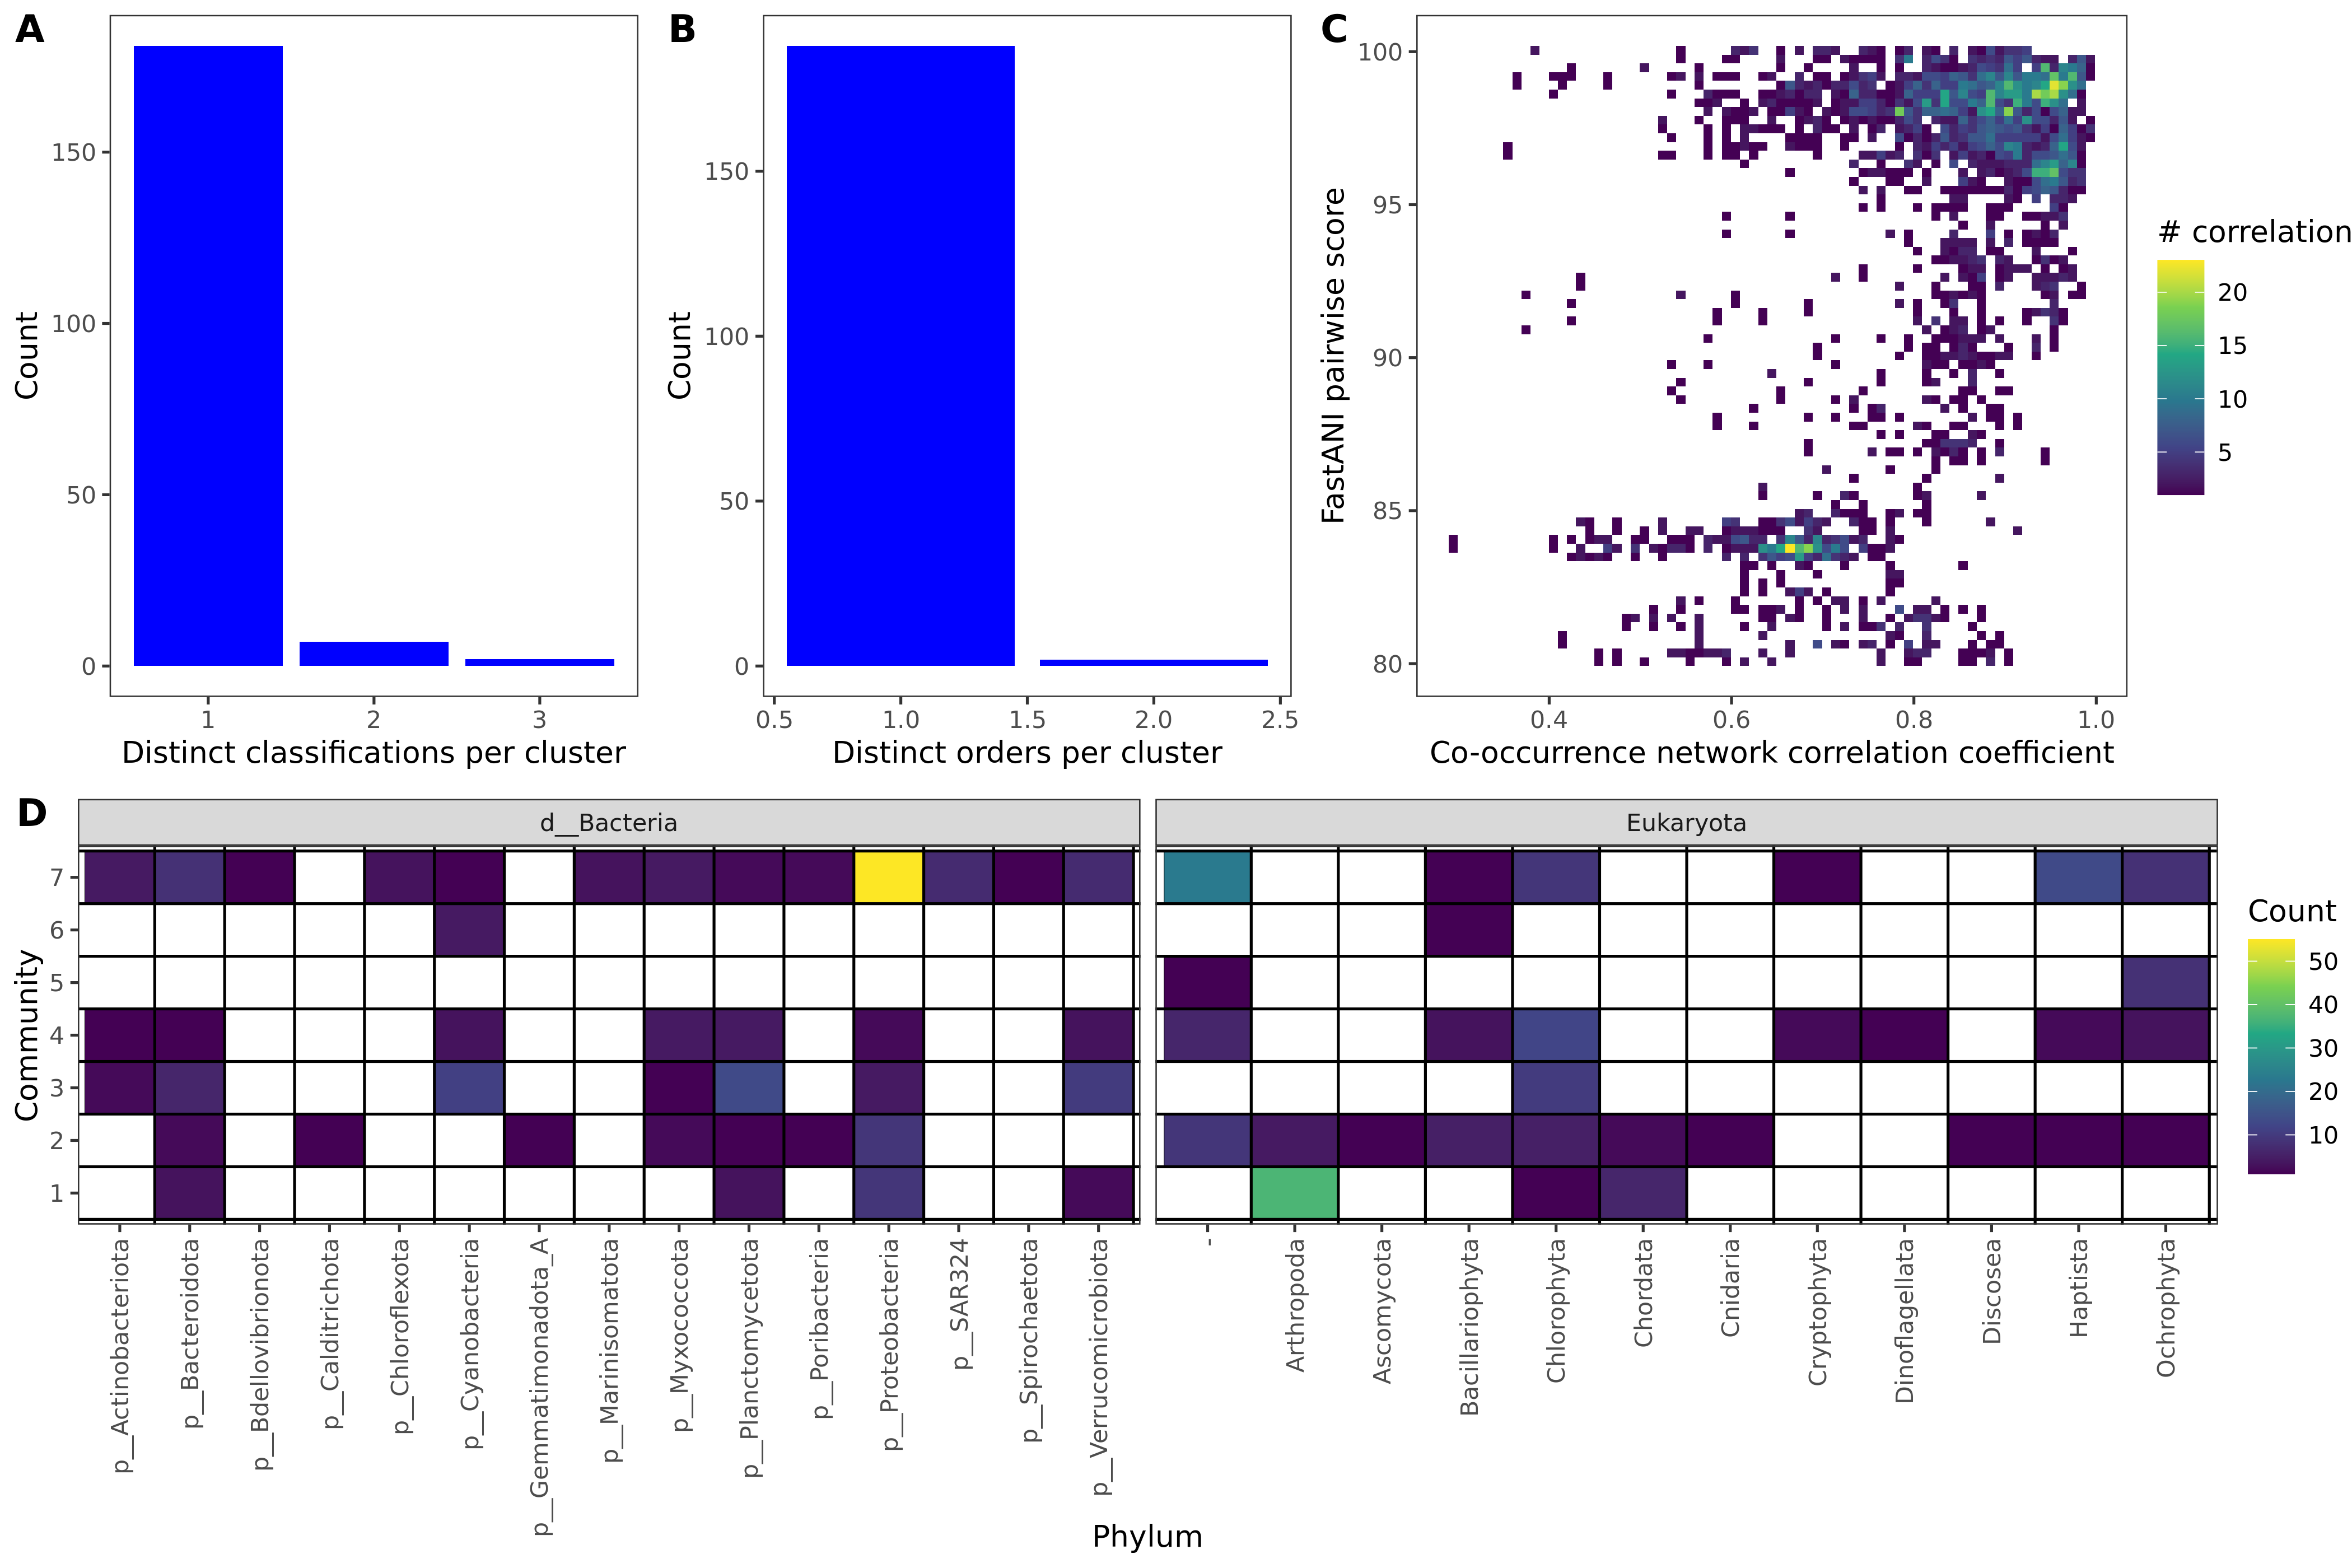
\includegraphics[width=0.95\columnwidth]{si-figures/network_supporting.png}
        \caption{Supporting figures for the network analysis section. A and B: FastANI clustering does not typically group together eukaryotic MAGs of different overall taxonomic classification (A) or taxonomic order (B). C: Justification for ANI cutoff of 95\% (and correlation coefficient 0.504) for considering eukaryotic MAGs to be sufficiently similar to be clustered. The majority of MAGs with pairwise ANI scores of $\geq$95 have correlation coefficiently of $\geq$0.8. D: Taxonomic composition of the 7 identified communities from the main text.}
        \label{fig:network-support}
    \end{figure}
\end{landscape}

\begin{landscape}
    \begin{figure}
        \centering
        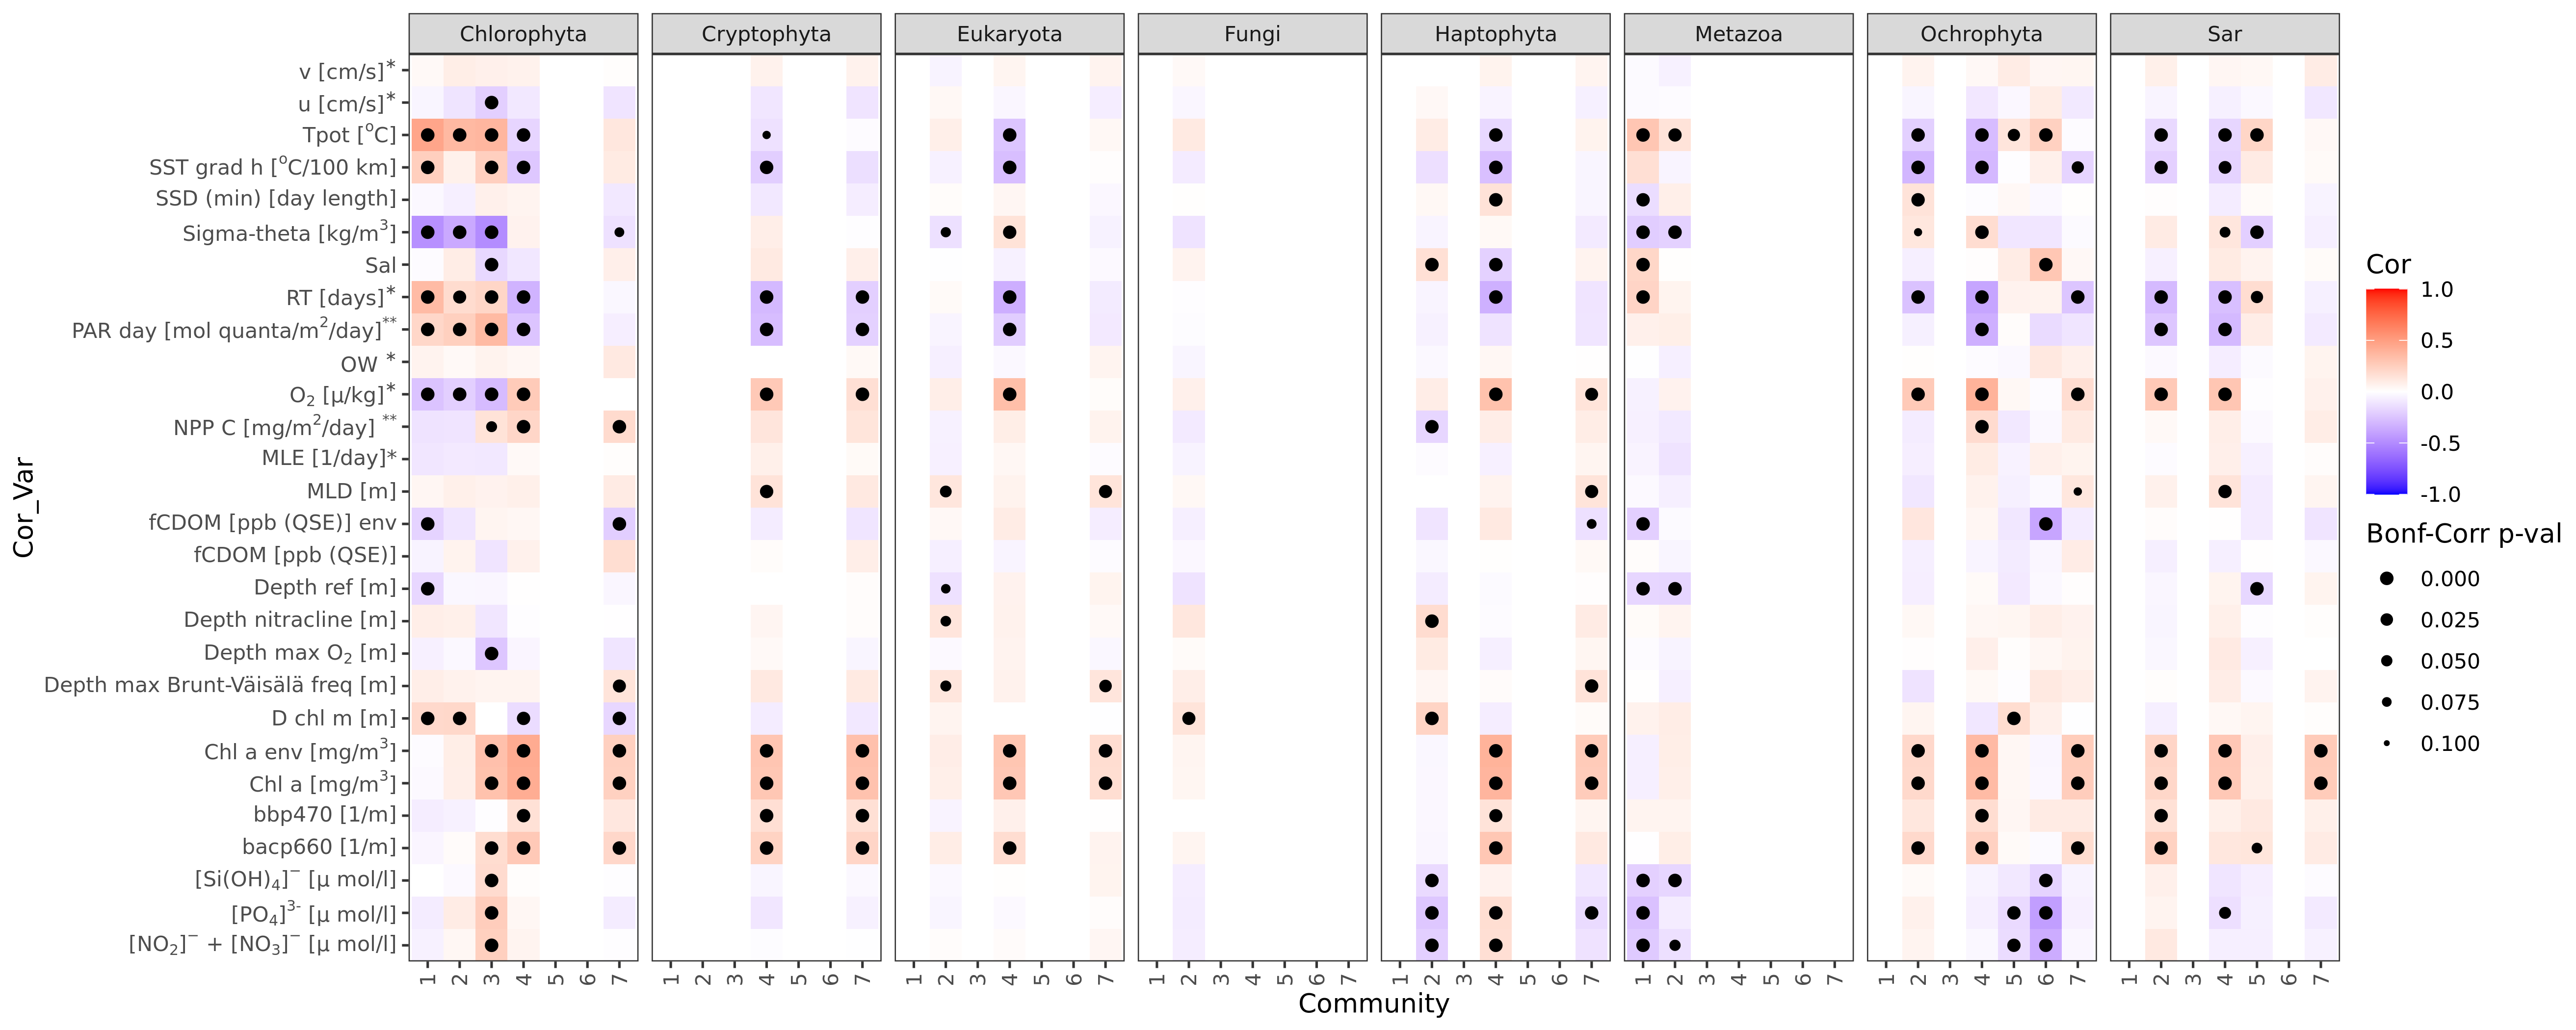
\includegraphics[width=0.95\columnwidth]{si-figures/bygroup.png}
        \caption{}
        \label{fig:network-bygroup}
    \end{figure}
\end{landscape}

\bibliographystyle{abbrvnat}

\bibliography{main}
\end{document}
